\documentclass[12pt]{article}
\usepackage[utf8x]{inputenc}
\usepackage{amsmath}
\usepackage{amsfonts}
\usepackage{mathrsfs}
\usepackage{natbib}
\usepackage{graphicx} % figuras
\usepackage[export]{adjustbox} % loads also graphicx
\usepackage{float}
\usepackage[font=footnotesize]{caption}
\usepackage{wrapfig}
\usepackage{authblk}
\usepackage{subfigure}
\usepackage{pifont}
\usepackage{a4wide}
%\usepackage{lipsum}
\topmargin=-2pt
\title{Physics-based pre-conditioners for large-scale subsurface flow simulation}

\author[1]{G. B. Diaz Cortes}  
\author[1]{C. Vuik} 
\author[2]{J. D. Jansen} 
\affil[1]{Department of Applied Mathematics, TU Delft}
\affil[2]{Department of Geoscience \& Engineering, TU Delft}
\renewcommand\Authands{ and }
\date{March 2016}
\begin{document}



% Title Page

\maketitle
\begin{abstract}
     We study fast and robust iterative solvers for large systems of  linear equations resulting from reservoir simulation trough porous media. We propose the use of preconditioning and deflation techniques based on information obtained from the system to reduce the time spent in the solution of the linear system.\\
 We consider compressible and incompressible single-phase flow in a layered model with large variations in the permeability coefficients and the SPE10 benchmark model (the Markovinovic problem).\\
\end{abstract}

  \section*{Introduction.}
  \hspace{0.5cm}Often, most computational time in the simulation of multi-phase flow through porous media is taken up by
solution of the pressure equation. This involves primarily solving large systems of linear equations as 
part of the iterative solution of the time and space discretized governing nonlinear partial differential 
equations. The time spent in solving the linear systems depends on the size of the problem and the 
variations of permeability within the medium. Solution of problems with extreme contrast in the grid block 
permeability values may lead to very large computing times.\\
A potential approach to reduce the computing time for large-scale problems with the aid of Proper Orthogonal 
Decomposition (POD) is investigated in \cite{Astrid11} and \cite{Mark06}. Astrid et al. \cite{Astrid11} 
propose the use of a POD-based preconditioner for the acceleration  of the solution to the pressure equation. 
The preconditioner is constructed from a set of snapshots, obtained from solutions to the pressure equation 
in previous time steps. Once the snapshots are computed, the POD method is used to obtain a set of basis 
vectors that capture the most relevant features of the system, which can be used to improve the simulation 
time of the subsequent time steps. A similar approach is used in \cite{Mark06}, where a set of POD-based 
basis vectors is obtained from the initial time steps. However, in this case, the acceleration is 
achieved by only improving the initial guess.\\
Problems with a high contrast between the permeability coefficients are sometimes approached through the 
use of deflation techniques; see, e.g., \cite{Vuik99}. The use of deflation techniques involves the search 
of good deflation vectors, which are usually problem-dependent. In \cite{Vuik99}, subdomain based deflation 
vectors are used for layered problems with a large contrast between the permeability coefficients. However, 
these deflation vectors cannot be used if the distribution of the permeability coefficients  is not 
structured as is the case in, e.g., the well-known SPE 10 benchmark problem \cite{Christie01}.\\
Following the ideas of \cite{Astrid11} and \cite{Mark06}, we propose the use of POD of many snapshots to capture 
the system's behavior. The basis obtained with POD is studied as an alternative choice of deflation vectors 
to accelerate the convergence of the pressure solution in a porous medium with high-contrast variations in the 
permeability coefficients. We consider incompressible and compressible single-phase flow through porous media 
with large variations in the permeability coefficients for layered academic problems and the SPE 10 benchmark (Markovinovic problem). 
\\


 In Section \ref{syseq} we give some theory about the linear solver used for this work and we introduce preconditioning and deflation techniques. We also demonstrate two lemmas that will help us in the choice of good deflation vectors for the incompressible case, necessary for the deflation techniques.\\
 In Section \ref{numexp} we present numerical experiments. We describe the problem that is studied, the solver that is used and the preconditioning and deflation techniques used for the speedup of the solver. The results are also presented in this section. \\
 Finally, we end with the conclusions.
\newpage
\section{Iterative solution methods}\label{syseq}
The solution of partial differential equations PDE's 
can be performed with numerical methods. Some of these methods, as the finite differences method, 
transform our equations into a linear 
system of the form:
\begin{gather*}
a_{11}x_{1}+\dots+a_{1n}x_{n}=b_{1},\\
\dots\\
a_{n1}x_{1}+....+a_{nn}x_{n}=b_{n},
\end{gather*}
which is written in matrix form as:
\begin{equation}\label{eq:linsys}
 \mathbf{A}\mathbf{x}=\mathbf{b}.
\end{equation}
System $\eqref{eq:linsys}$ can be solved with direct or iterative methods. Direct methods achieve a final solution, 
while the iterative ones
are stopped if the error is less than a given value. \\
Some of the iterative methods are: Jacobi, Gauss Seidel, and if the
matrix is Symetric Positive Definite $SPD$\footnote{$\mathbf{A}^T=\mathbf{A},$ and $(\mathbf{A}\mathbf{x},\mathbf{x})>0, \qquad \forall \mathbf{x} \in \mathbb{R}^n, \qquad \mathbf{x}\neq0.$} we can use the Conjugate Gradient (CG) method.
This section is devoted to iterative methods, in particular CG, that is the
method used in this work. \\
In this section, we also describe the Preconditioning and Deflation techniques 
for the acceleration of the CG method.
\subsection{Krylov subspace Methods}
If we have two subspaces $\mathcal{K}_k,$ $\mathcal{L}_k$ of $\mathbb{R}^n$ and we want to solve 
the Equation \eqref{eq:linsys}, 
with $\mathbf{A} \in \mathbb{R}^{n\times n}$ we can use a projection method onto $\mathcal{K}_k$.
This method allows us to find an approximate solution $\mathbf{x}^k$ from an arbitrary initial guess 
solution $\mathbf{x}^0$. This approximate solution lies in the Krylov subspace of dimension $k$ of the matrix $\mathbf{A}$ 
and residual $\mathbf{r}^0$,
\begin{equation*}
\mathbf{x}^k \in \mathbf{x}^0+\mathcal{K}_k(\mathbf{A},\mathbf{r}^0),
\end{equation*}
with $\mathcal{K}_k(\mathbf{A},\mathbf{r}^0)$ defined as:
\begin{equation*}
\mathcal{K}_k(\mathbf{A},\mathbf{r}^0)=span\{\mathbf{r}^0,\mathbf{A}\mathbf{r}^0,\dots,\mathbf{A}^{k-1}\mathbf{r}^0\}.
\end{equation*}
Where the residual $\mathbf{r}^k=\mathbf{b}-\mathbf{A}\mathbf{x}^k$ is orthogonal to the subspace $\mathcal{L}_k$, with 
\begin{equation*}
 \mathbf{x}^{k+1}=\mathbf{x}^k+\mathbf{B}^{-1}r^k, \qquad \mathbf{r}^k=\mathbf{b}-\mathbf{A}\mathbf{x}^k.
\end{equation*}
The subspace $\mathcal{L}_k$ is chosen depending on the Krylov subspace method that is used.


\subsection{Conjugate Gradient Method}
\hspace{0.5cm}The Conjugate Gradient (CG) method is a Krylov subspace method for $SPD$ matrices, such that
\begin{equation}\label{eq:CGm}
 ||\mathbf{x}-\mathbf{x}^k||_\mathbf{A} \footnote{$||\mathbf{x}||_\mathbf{A}= \sqrt{(\mathbf{x},\mathbf{x})_\mathbf{A}}=\sqrt{\mathbf{x}^T\mathbf{A}\mathbf{x}}.$} 
\end{equation}
is minimal, with $\mathbf{x}$ the solution of the system and $\mathbf{x}^k$ the approximate solution
after $k$ iterations and the error of this iteration is bounded by:
\begin{equation}\label{eq:conv}
 ||\mathbf{x}-\mathbf{x}^{k}||_\mathbf{A}\leq 2||\mathbf{x}-\mathbf{x}^{0}||_\mathbf{A} 
 \left( \frac{\sqrt{\mathbf{\kappa}_2(\mathbf{A})}-1}{\sqrt{\mathbf{\kappa}_2(\mathbf{A})}+1} \right)^{k}.
 \footnote{The condition number $\mathbf{\kappa}_2(\mathbf{A})$ is defined as  $\mathbf{\kappa}_2(\mathbf{A})=
 \frac{\sqrt{\lambda_{max}(\mathbf{A}^T\mathbf{A})}}{\sqrt{\lambda_{min}(\mathbf{A}^T\mathbf{A})}}$. 
 If $\mathbf{A}$ is SPD, $\mathbf{\kappa}_2(\mathbf{A})=\frac{\lambda_{max}(\mathbf{A})}{\lambda_{min}(\mathbf{A})}$.}
 \end{equation} \\

\begin{table}[!h]
\begin{tabular}{ |l| } 
\hline
  \textbf{Algorithm 1} Conjugate Gradient (CG) method, solving $\mathbf{A}\mathbf{x}=\mathbf{b}$.\\
  \hline
 \hline
\\
Give an initial guess $\mathbf{x}^0$. \\Compute $\mathbf{r}^0=\mathbf{b}-\mathbf{A}\mathbf{x}^0$ and set $\mathbf{p}^0=\mathbf{r}^0$.\\

\hspace{0.5cm}\textbf{for} $k=0,...,$ until convergence\\
 \hspace{1cm} $\alpha^k=\frac{(\mathbf{r}^{k},\mathbf{r}^{k})}{(\mathbf{A}\mathbf{p}^k,\mathbf{p}^k)}$\\
\hspace{1cm} $\mathbf{x}^{k+1}=\mathbf{x}^k+\alpha^k\mathbf{p}^k$\\
\hspace{1cm}$\mathbf{r}^{k+1}=\mathbf{r}^k-\alpha^k\mathbf{A}\mathbf{p}^k$\\
\hspace{1cm}$ \beta^k=\frac{(\mathbf{r}^{k+1},\mathbf{r}^{k+1})}{(\mathbf{r}^k,\mathbf{r}^k)}$\\
\hspace{1cm}$\mathbf{p}^{k+1}=\mathbf{r}^{k+1}+\beta^k\mathbf{p}^k$\\
\hspace{0.5cm}\textbf{end}\\
\hline
\end{tabular}
\end{table}
 
 \subsection{Preconditioning}
\hspace{0.5cm}If we want to accelerate the convergence of an iterative method, we can transform the system into
another one containing a better spectrum, i.e, a smaller condition number. 
This can be done by multiplying the original system \eqref{eq:linsys} by a matrix $\mathbf{M}^{-1}.$
\begin{equation}\label{eq:precon}
 \mathbf{M}^{-1}\mathbf{A}\mathbf{x}=\mathbf{M}^{-1}\mathbf{b}.
\end{equation}
The new system has the same solution but provides a substantial improvement on the spectrum. 
For this preconditioned system, the convergence is given by:
\begin{equation}\label{eq:convp}
 ||\mathbf{x}-\mathbf{x}^{k+1}||_\mathbf{A}\leq 2||\mathbf{x}-\mathbf{x}^{0}||_\mathbf{A} 
 \left( \frac{\sqrt{\mathbf{\kappa}(\mathbf{M}^{-1}\mathbf{A})}-1}{\sqrt{\mathbf{\kappa}(\mathbf{M}^{-1}\mathbf{A})}+1} \right)^{k+1}.
\end{equation}
$\mathbf{M}$ is an $SPD$ matrix chosen such that $\mathbf{\kappa}(\mathbf{M}^{-1}\mathbf{A})\leq \mathbf{\kappa}(\mathbf{A}),$ and $\mathbf{M}^{-1}b$ is easy to compute.
The Conjugate Gradient (CG) method is a Krylov subspace method for Symmetric Positive Definite $SPD$ matrices, such that
\begin{equation}\label{eq:CGm}
 ||\mathbf{x}-\mathbf{x}^k||_\mathbf{A}, \footnote{$||\mathbf{x}||_\mathbf{A}= \sqrt{(\mathbf{x},\mathbf{x})_\mathbf{A}}=\sqrt{\mathbf{x}^T\mathbf{A}\mathbf{x}}.$} 
\end{equation}
is minimal, with $\mathbf{x}$ the solution of the system and $\mathbf{x}^k$ the $k-th$ iteration. \\
Given an initial guess $\mathbf{x}^0$ the next approximations can be computed following the search directions $\mathbf{p}^i$ 
$$\mathbf{x}^{k+1}=\mathbf{x}^k+\alpha^k\mathbf{p}^k.$$ 
For the CG method, the search directions $\mathbf{p}^k$ are orthogonal with 
respect to the $\mathbf{A}$ inner product, i.e.
$$(\mathbf{A}\mathbf{p}^k,\mathbf{p}^j)=0, \qquad k\neq j,$$
and the residuals form an orthogonal set, i.e.
$$(\mathbf{r}^k,\mathbf{r}^j)=0, \qquad k \neq j.$$
The constant $\alpha^k$ that satisfies \eqref{eq:CGm} is given by:
$$\alpha^k=\frac{(\mathbf{r}^{k},\mathbf{r}^{k})}{(\mathbf{A}\mathbf{p}^k,\mathbf{p}^k)},$$
and the new search directions can be computed via the residuals,
$$\mathbf{p}^{k+1}=\mathbf{r}^{k+1}+\beta_k\mathbf{p}^k,$$
where 
$$ \beta_k=\frac{(\mathbf{r}^{k+1},\mathbf{r}^{k+1})}{(\mathbf{r}^k,\mathbf{r}^k)}.$$
After $k+1$ iterations of the $CG$ method, the error of the iteration will be bounded by:
\begin{equation}\label{eq:conv}
 ||\mathbf{x}-\mathbf{x}^{k+1}||_\mathbf{A}\leq 2||\mathbf{x}-\mathbf{x}^{0}||_\mathbf{A} 
 \left( \frac{\sqrt{\kappa_2(\mathbf{A})}-1}{\sqrt{\kappa_2(\mathbf{A})}+1} \right)^{k+1}
 \footnote{The condition number $\kappa_2(\mathbf{A})$ is defined as  $\kappa_2(\mathbf{A})=
 \frac{\sqrt{\lambda_{max}(\mathbf{A}^T\mathbf{A})}}{\sqrt{\lambda_{min}(\mathbf{A}^T\mathbf{A})}}$. 
 If $\mathbf{A}$ is SPD, $\kappa_2(\mathbf{A})=\frac{\lambda_{max}(\mathbf{A})}{\lambda_{min}(\mathbf{A})}$.}.
 \end{equation}
 
\subsection{Deflation}\label{def}
\hspace{0.5cm}Deflation is used to annihilate the effect of extreme eigenvalues on the convergence of an iterative method (\cite{Vuik99}). 
Given an $SPD$ matrix $\mathbf{A} \in \mathbb{R}^{n \times n}$, the deflation matrix $\mathbf{P}$ is defined as follows (\cite{Tang08}):
$$\mathbf{P}=\mathbf{I}-\mathbf{A}\mathbf{Q}, \qquad \mathbf{P} \in \mathbb{R}^{n \times n}, \qquad \mathbf{Q} \in \mathbb{R}^{n \times n},$$
where
$$\mathbf{Q}=\mathbf{Z}\mathbf{E}^{-1}\mathbf{Z}^T, \qquad \mathbf{Z} \in \mathbb{R}^{n \times m}, \qquad \mathbf{E} \in \mathbb{R}^{m \times m}, $$
with
$$\mathbf{E}=\mathbf{Z}^T\mathbf{A}\mathbf{Z}.$$
The matrix $\mathbf{E}$ is known as the $Galerkin$ or $coarse$ matrix that has to be invertible. 
If $\mathbf{A}$ is $SPD$ and $\mathbf{Z}$ is full rank then $\mathbf{E}$ is invertible. 
The full rank matrix $\mathbf{Z}$ is called the $deflation-subspace$ matrix, 
and it's $l<n$ columns are the
$deflation$ vectors or $projection$ vectors.\\
Some properties of the previous matrices are (\cite[pag. 27]{Tang08}):
\begin{enumerate}\label{defprop}
 \item[a)] $\mathbf{P}^2=\mathbf{P}.$
 \item[b)] $\mathbf{A}\mathbf{P}^T=\mathbf{P}\mathbf{A}.$
 \item[c)] $(\mathbf{I}-\mathbf{P}^T)\mathbf{x}=\mathbf{Q}\mathbf{b}.$
 \item[d)] $\mathbf{P}\mathbf{A}\mathbf{Z}=\mathbf{0}^{n\times m}.$
 \item[e)] $\mathbf{P}\mathbf{A}$ is $SPSD$\footnote{Symmetric Positive Semi-Definite, $(\mathbf{A}\mathbf{x},\mathbf{x})\geq 0$, for all $\mathbf{x}$.}.
\end{enumerate}
We can split the vector $\mathbf{x}$ as:
\begin{equation}\label{eq:splx}
    \mathbf{x}=\mathbf{I}\mathbf{x}-\mathbf{P}^T\mathbf{x}+\mathbf{P}^T\mathbf{x}=(\mathbf{I}-\mathbf{P}^T)\mathbf{x}+\mathbf{P}^T\mathbf{x}.
\end{equation}
Multiplying the expression above by $\mathbf{A}$, using the properties above, we have:
\begin{align*}
\mathbf{A}\mathbf{x}&=\mathbf{A}(\mathbf{I}-\mathbf{P}^T)\mathbf{b}+\mathbf{A}\mathbf{P}^T\mathbf{x},\qquad&Property:\\
\mathbf{A}\mathbf{x}&=\mathbf{A}\mathbf{Q}\mathbf{b}+\mathbf{A}\mathbf{P}^T\mathbf{x},&c)\\
\mathbf{b}&=\mathbf{A}\mathbf{Q}\mathbf{b}+\mathbf{P}\mathbf{A}\mathbf{x},&b),
\end{align*}
multiplying by $\mathbf{P}$ and using the properties $\mathbf{P}\mathbf{A}\mathbf{Q}=
\mathbf{0}^{n\times n}$ and $\mathbf{P}^2=\mathbf{P}$, properties $d$) and $e$), we have:
\begin{align}\label{eq:defsys}
\mathbf{P}\mathbf{A}\mathbf{Q}\mathbf{b}+\mathbf{P}^2\mathbf{A}\mathbf{x}&=\mathbf{P}\mathbf{b},\nonumber \\
\mathbf{P}\mathbf{A}\mathbf{x}&=\mathbf{P}\mathbf{b},
\end{align}
where $\mathbf{P}\mathbf{A}\mathbf{x}=\mathbf{P}\mathbf{b}$ is the deflated system. Since 
$\mathbf{P}\mathbf{A}$ is singular, the solution $\mathbf{x}$ can contain
components of the null space of $\mathbf{P}\mathbf{A}$. A solution to this system, called deflated
solution, is denoted by $\mathbf{\hat{x}}$.
The deflated system for $\mathbf{\hat{x}}$ is:
\begin{align}\label{eq:defsol}
\mathbf{P}\mathbf{A} \hat{\mathbf{x}}=\mathbf{P}\mathbf{b}.
\end{align}
As mentioned above, the solution to Equation \eqref{eq:defsys} can contain components of 
$\mathcal{N}(\mathbf{P}\mathbf{A})$. Therefore, a solution to Equation \eqref{eq:defsol},
$\mathbf{\hat{x}}$ can be decomposed as:
\begin{equation}\label{eq:xxy}
\mathbf{\hat{x}}=\mathbf{x}+ \mathbf{y},
\end{equation}
with $\mathbf{y} \in \mathcal{R}(\mathbf{Z})\subset \mathcal{N}(\mathbf{P}\mathbf{A}),$ 
and $\mathbf{x}$ the solution to Equation \eqref{eq:linsys}.\\
Note: If $\mathbf{y} \in \mathcal{R}(\mathbf{Z}),$ then $$\mathbf{y}=\sum^{m}_{i=1}\alpha_i \mathbf{z}_i,$$\\
 \begin{equation}\label{eq:paz}
 \mathbf{P}\mathbf{A}y=\mathbf{P}\mathbf{A}(\mathbf{z}_1\alpha_1 +...+ \mathbf{z}_m\alpha_m)=\mathbf{P}\mathbf{A}\mathbf{Z}\mathbf{\alpha},\end{equation}
 from \ref{defprop} h) $\mathbf{P}\mathbf{A}\mathbf{Z}=\mathbf{0}^{n\times l},$ then 
 \begin{equation}\label{eq:pay}
 \mathbf{P}\mathbf{A}\mathbf{y}=\mathbf{0}.
 \end{equation}
Therefore $\mathcal{R}(\mathbf{Z})\subset \mathcal{N}(\mathbf{P}\mathbf{A}).$ \\
Multiplying Equation \eqref{eq:xxy} by $\mathbf{P}^T$ we obtain:
$$\mathbf{P}^T\mathbf{\hat{x}}=\mathbf{P}^T\mathbf{x}+\mathbf{P}^T\mathbf{y},$$
combining Equation \eqref{eq:pay} with \ref{defprop} f), we have:
 \begin{equation*}
 \mathbf{P}\mathbf{A}y=\mathbf{A}\mathbf{P}^T\mathbf{y}=\mathbf{0}.
 \end{equation*}
 Therefore
  \begin{equation}\label{eq:ptx}
\mathbf{P}^T\mathbf{\hat{x}}=\mathbf{P}^T\mathbf{x}.
 \end{equation}
Substitution to Equation \eqref{eq:ptx} and \ref{defprop} g) in Equation \eqref{eq:splx} leads to:
\begin{equation}\label{eq:xfromxh}
    \mathbf{x}=\mathbf{Q}\mathbf{b}+\mathbf{P}^T\mathbf{\hat{x}}, 
\end{equation}
which gives us a relation between $\mathbf{\hat{x}}$ and $\mathbf{x}$.
 
\subsection{Deflated CG Method}
\hspace{0.5cm}To obtain the solution to the linear system \eqref{eq:linsys}, we solve the deflated system:
\begin{equation}\label{eq:deflsys}
    \mathbf{P}\mathbf{A}\hat{\mathbf{x}}=\mathbf{P}\mathbf{b}.
\end{equation}
with the CG method, for a deflated solution $\hat{\mathbf{x}}$. 
Therefore, the solution $\mathbf{x}$ to the original system is obtained from \eqref{eq:xfromxh}:
$$\mathbf{x}=\mathbf{Q}\mathbf{b}+\mathbf{P}^T\hat{\mathbf{x}}.$$
\subsection*{Deflated PCG Method}
The deflated linear system can also be preconditioned by an $SPD$ matrix $\mathbf{M}$.\\
The deflated preconditioned system to solve with CG is \cite[pag. 30]{Tang08}:
$$\tilde{\mathbf{P}} \tilde{\mathbf{A}} \hat{\tilde{\mathbf{x}}}=\tilde{\mathbf{P}}\tilde{\mathbf{b}},$$
where:
\begin{equation*}
 \tilde{\mathbf{A}}=\mathbf{M}^{-\frac{1}{2}}\mathbf{A}\mathbf{M}^{-\frac{1}{2}}, \qquad \hat{\tilde{\mathbf{x}}}=\mathbf{M}^{\frac{1}{2}}\hat{\mathbf{x}}, \qquad
 \tilde{\mathbf{b}}=\mathbf{M}^{-\frac{1}{2}}\mathbf{b}
\end{equation*}
This method is called the Deflated Preconditioned Conjugate Gradient $DPCG$ method, and the error is bounded by:
\begin{equation*}
 ||\mathbf{x}-\mathbf{x}^{i+1}||_\mathbf{A}\leq 2||\mathbf{x}-\mathbf{x}^{0}||_\mathbf{A} \left( \frac{\sqrt{\mathbf{\kappa}_{eff}(\mathbf{M}^{-1}\mathbf{P}\mathbf{A})}-1}{\sqrt{\mathbf{\kappa}_{eff}(\mathbf{M}^{-1}\mathbf{P}\mathbf{A})}+1} \right)^{i+1},
\end{equation*}
were $\mathbf{C}_{eff}=\frac{\lambda_{max}(M^{-1}PA)}{\lambda_{min}(M^{-1}PA)}$ is the effective condition 
number and $\lambda_{min}(M^{-1}PA)$ is the smallest non-zero eigenvalue of $M^{-1}PA$.
\subsection{Choices of Deflation Vectors}
\hspace{0.5cm}The deflation method is used to treat the most unfavorable eigenvalues
of $\mathbf{A}$. If the matrix $\mathbf{Z}$ contains eigenvectors corresponding to the unfavorable 
eigenvalues, the convergence of the 
iterative method is achieved faster. However, to obtain and to apply the eigenvectors is costly in most 
of the cases.
Therefore, a good choice of the matrix $\mathbf{Z}$ that does not contain the eigenvectors is essential
for the acceleration of the convergence.\\
A good choice of the deflation vectors is usually problem-dependent. Available information on the system is, in general,
used to obtain these vectors.
Most of the techniques used to choose deflation vectors are based on approximating eigenvectors, 
recycling (\cite{Clemens04}), subdomain deflation vectors (\cite{Vuik02}) or multigrid and 
multilevel based deflation techniques (\cite{Tang09,Smith96}). A summary of these techniques is given below.
\begin{description}
 \item [Recycling Deflation.] A set of vectors previously used is reused to build the deflation-subspace 
 matrix (\cite{Clemens04}). 
The vectors could be, for example, $q-1$
solution vectors of the linear system with different right-hand sides or of different time steps.
The matrix $\mathbf{Z}$ containing this solutions is:
$$\mathbf{Z}=[\mathbf{x}^{(1)},\mathbf{x}^{(2)},...,\mathbf{x}^{(q-1)}].$$
 \item [Subdomain Deflation.] The domain is divided into several subdomains,
 each corresponding to one or more deflation vectors.
For each subdomain, there is a deflation vector that has ones for points in the 
subdomain and zeros for points outside (\cite{Vuik02}).
 \item [Multi Grid and Multilevel Deflation.] For the multigrid and multilevel methods, 
 there are matrices called prolongation and restriction matrices that
allow us to pass from one level or grid to another. 
These matrices are used as the deflation-subspace matrices $\mathbf{Z}$ (\cite{Tang09}).
\end{description}



\subsection{Analysis of the snapshots}
As mentioned in the previous section, it is important to choose 'good' deflation vectors if we want to
obtain a speedup of an iterative method.\\ 
We can use solutions of a system slightly different from the original (snapshots) as deflation vectors.
For this, we need to choose the way of selecting these snapshots
wisely. The idea behind this selection is to obtain a small number of snapshots and at the same time
obtain the largest amount of information from the system.\\
In this section two lemmas are proved. The lemmas could help us to select the systems that we are going to solve for
the snapshots.\\\\
\textbf{Lemma 1.} 
Let $\mathbf{A} \in \mathbb{R}^{n\times n}$ be a non-singular matrix, such that
\begin{equation}\label{eq:ls}
\mathbf{A}\mathbf{x}=\mathbf{b},
\end{equation}
and $ \mathbf{x}_i, \mathbf{b}_i \in \mathbb{R}^{n},$ $i=1,...,m,$ where the vectors $\mathbf{b}_i$ are 
linearly independent ($l.i.$) such that: 
\begin{equation}\label{eq:lieq}
\mathbf{A}\mathbf{x}_i=\mathbf{b}_i,
\end{equation}
The following equivalence holds
\begin{equation}\label{eq:equiv}
\mathbf{x}=\sum_{i=1}^m {c}_i\mathbf{x}_i \qquad
\Leftrightarrow \qquad
\mathbf{b}=\sum_{i=1}^m {c}_i\mathbf{b}_i.
\end{equation}
Proof $\Rightarrow$
\begin{equation}\label{eq:equiv1}
\mathbf{x}=\sum_{i=1}^m {c}_i\mathbf{x}_i 
\Rightarrow 
\mathbf{b}=\sum_{i=1}^m {c}_i\mathbf{b}_i.
\end{equation}
Substituting $\mathbf{x}$ from \eqref{eq:equiv1} into $\mathbf{A}\mathbf{x}=\mathbf{b}$ leads to:
\begin{align*}
\mathbf{A}\mathbf{x}&=\sum_{i=1}^m \mathbf{A}{c}_i\mathbf{x}_i=\mathbf{A}(c_1\mathbf{x}_1+...+c_m\mathbf{x}_m).
\end{align*}
Using the linearity of $\mathbf{A}$ the equation above can be rewritten as:
\begin{align}\label{eq:bc}
\mathbf{A}c_1\mathbf{x}_1+...+\mathbf{A}c_m\mathbf{x}_m
=c_1\mathbf{b}_1+...+c_m\mathbf{b}_m=\mathbf{B}\mathbf{c}.
\end{align}
where $\mathbf{B} \in \mathbb{R}^{n\times m},$ $\mathbf{c} \in \mathbb{R}^{m}$, and the columns of $\mathbf{B}$
are the vectors $\mathbf{b}_i$.\\
From \eqref{eq:ls} and \eqref{eq:bc} we get:
\begin{align*}
\mathbf{A}\mathbf{x}=\mathbf{b}=c_1\mathbf{b}_1+...+c_m\mathbf{b}_m=\sum_{i=1}^m {c}_i\mathbf{b}_i.\\
\end{align*}
Proof $\Leftarrow $
\begin{equation}\label{eq:equiv2}
\mathbf{x}=\sum_{i=1}^m {c}_i\mathbf{x}_i\Leftarrow \mathbf{b}=\sum_{i=1}^m {c}_i\mathbf{b}_i .
\end{equation}
Substituting $\mathbf{b}$ from \eqref{eq:equiv2} into $\mathbf{A}\mathbf{x}=\mathbf{b}$ leads to:
\begin{align}\label{eq:equiv21}
\mathbf{A}\mathbf{x}&=\sum_{i=1}^m {c}_i\mathbf{b}_i.
\end{align}
Since $\mathbf{A}$ is non-singular, multiplying \eqref{eq:lieq} and \eqref{eq:equiv2} by $\mathbf{A}^{-1}$ we obtain:
\begin{align}\label{eq:equiv21}
\mathbf{x}_i&=\mathbf{A}^{-1}\mathbf{b}_i,
\end{align}
\begin{align}\label{eq:equiv21}
\mathbf{x}&=\mathbf{A}^{-1}\sum_{i=1}^m {c}_i\mathbf{b}_i=\sum_{i=1}^m {c}_i\mathbf{A}^{-1}\mathbf{b}_i=\sum_{i=1}^m {c}_i\mathbf{x}_i.
\end{align}
\begin{flushright}
$Q.E.D.$                  
\end{flushright}
\textbf{Lemma 2.}
If the the deflation matrix $\mathbf{Z}$ is constructed with a set of $m$ vectors 
\begin{equation}
 \mathbf{Z}=
\begin{bmatrix}
\mathbf{x}_1&...&...&\mathbf{x}_m
\end{bmatrix}, 
\end{equation}
such that $\mathbf{x}=\sum_{i=1}^m {c}_i\mathbf{x}_i$, with $\mathbf{x}_i$ $l.i.$, then the solution of
system $\mathbf{A}\mathbf{x}=\mathbf{b}$ is achieved within one iteration of DCG.\\
Proof.\\
The relation between $\mathbf{\hat{x}}$ and $\mathbf{x}$ is given in Equation \eqref{eq:xfromxh}:
\begin{equation*}
    \mathbf{x}=\mathbf{Q}\mathbf{b}+\mathbf{P}^T\mathbf{\hat{x}}. 
\end{equation*}
For the first term $\mathbf{Q}\mathbf{b}$, taking $\mathbf{b}=\sum_{i=1}^m {c}_i\mathbf{b}_i$ we have:

\begin{align*}
\mathbf{Q}\mathbf{b}&=\mathbf{Z}\mathbf{E}^{-1}\mathbf{Z}^T\left(\sum_{i=1}^m {c}_i\mathbf{b}_i\right)\\
&=\mathbf{Z}(\mathbf{Z}^T\mathbf{A}\mathbf{Z})^{-1}\mathbf{Z}^T\left(\sum_{i=1}^m {c}_i\mathbf{A}\mathbf{x}_i\right)\qquad \text{using Lemma 1}\\
&=\mathbf{Z}(\mathbf{Z}^T\mathbf{A}\mathbf{Z})^{-1}\mathbf{Z}^T\left( \mathbf{A}\mathbf{x}_1{c}_1+...+\mathbf{A}\mathbf{x}_m{c}_m\right) \\
&=\mathbf{Z}(\mathbf{Z}^T\mathbf{A}\mathbf{Z})^{-1}\mathbf{Z}^T(\mathbf{A}\mathbf{Z}\mathbf{c})  \\
&=\mathbf{Z}(\mathbf{Z}^T\mathbf{A}\mathbf{Z})^{-1}(\mathbf{Z}^T\mathbf{A}\mathbf{Z})\mathbf{c} \\
&=\mathbf{Z}\mathbf{c}= c_1\mathbf{x}_1+c_2\mathbf{x}_2+c_3\mathbf{x}_3+c_4\mathbf{x}_4+c_5\mathbf{x}_5\\
& =\sum_{i=1}^m {c}_i\mathbf{x}_i=\mathbf{x},
\end{align*}
\\
which is the solution of the original system.\\ 
For the second term of Equation \eqref{eq:xfromxh}, $\mathbf{P}^T\mathbf{\hat{x}}$, we compute $\mathbf{\hat{x}}$ from Equation \eqref{eq:deflsys}:
\begin{align*}
    \mathbf{P}\mathbf{A}\hat{\mathbf{x}}&=\mathbf{P}\mathbf{b}\\
    \mathbf{A}\mathbf{P}^T\hat{\mathbf{x}}&=(\mathbf{I}-\mathbf{A}\mathbf{Q})\mathbf{b} \qquad \text{using \ref{defprop} f) and definition of $\mathbf{P}$,}\\
        \mathbf{A}\mathbf{P}^T\hat{\mathbf{x}}&=\mathbf{b}-\mathbf{A}\mathbf{Q}\mathbf{b}\\
        \mathbf{A}\mathbf{P}^T\hat{\mathbf{x}}&=\mathbf{b}-\mathbf{A}\mathbf{x}=0 \qquad \text{taking $\mathbf{Q}\mathbf{b}=\mathbf{x}$ from above,}\\
          \mathbf{P}^T\hat{\mathbf{x}}&=0 \qquad \text{as $\mathbf{A}$ is invertible.}
\end{align*}
Then we have achieve the solution $\mathbf{x}$ in one step of DICCG.\\


\subsubsection{Accuracy of the snapshots.}\label{accs}

If we use an iterative method to obtain an approximate solution $\mathbf{x}^k$, for the system $\mathbf{A}\mathbf{x}=\mathbf{b},$ we cannot compute the relative error of the approximation with respect to the true solution, 
$$\frac{||\mathbf{x}-\mathbf{x}^k||_2}{||\mathbf{x}||_2}.$$
Instead, we compute the relative residual, $$ \frac{||\mathbf{r}^k||_2}{||\mathbf{b}||_2}\leq \epsilon,$$
and we set a stopping criterium $\epsilon$ or tolerance, that is related to the relative error as follows (see Appendix \ref{a2}),
$$\frac{||\mathbf{x}-\mathbf{x}^k||_2}{||\mathbf{x}||_2}\leq \kappa_2(\mathbf{A}) \epsilon=\varepsilon,$$
where $\kappa_2(\mathbf{A})$ is the condition number of the matrix $\mathbf{A}$\\
Diverse tolerance values can be used in the experiments for the snapshots as well as for the solution of the original system. \\
If the maximum residual for the snapshots is $\epsilon=10^{-\eta}$ then the error of the snapshots is given by
$$\frac{||\mathbf{x}_i-\mathbf{x}_i^k||_2}{||\mathbf{x}_i||_2}\leq \kappa_2(\mathbf{A})\times 10^{-\eta}=\varepsilon.$$
If we use $m$ snapshots obtained with an iterative method to compute the solution of $\mathbf{x}$, after one iteration of DCG we obtain
$$\hat{x}=\sum_{i=1}^m {c}_i\mathbf{x}_i^{k(i)}.$$
The error of this solution is given by:
$$\frac{||\mathbf{x}-\mathbf{x}^k||_2}{||\mathbf{x}||_2}=
\frac{||\sum_{i=1}^m {c}_i(\mathbf{x}_i-\mathbf{x}_i^{k})||_2}{||\sum_{i=1}^m {c}_i\mathbf{x}_i||_2}\leq
\frac{\sum_{i=1}^m| {c}_i|\times \kappa_2(\mathbf{A})\times 10^{-\eta}}{||\sum_{i=1}^m {c}_i\mathbf{x}_i||_2}.
$$
Which means that the approximation has an error of $\mathcal{O}(\kappa_2\times10^{-\eta}).$
\\From Lemma 2 we know that if we use the snapshots $\mathbf{x}_i$ as deflation vectors, for the deflation method $$\mathbf{Q}\mathbf{b}=\mathbf{x}.$$ 
If the approximation has an error $\mathcal{O}(\kappa_2\times10^{-\eta})$, then the solution achieved with deflation will have the same error, 
$$\mathbf{Q}\mathbf{b}=\mathbf{x}^k+\mathcal{O}(\kappa_2\times10^{-\eta}).$$
Therefore, is important to take into account the condition number of the matrix related to the system  and the accuracy of the deflation vectors.
\subsubsection{Boundary conditions.}
From Lemma 2, we know that if we use as deflation vectors a set of $m$ snapshots $$\mathbf{Z}=[\mathbf{x}_1\qquad ...\qquad \mathbf{x}_m],$$ such that $\mathbf{x}=\sum_{i=1}^m {c}_i\mathbf{x}_i$, where $\mathbf{x}$ is the solution of the system $\mathbf{A}\mathbf{x}=\mathbf{b}$, the solution of the latter system is achieved within one iteration of DICCG. \\
In our application, only a small number ($m$) of elements of the right hand side vector ($\mathbf{b}$)
are changed for various situations. This implies that every $\mathbf{b}$ can be written as $\mathbf{b}=\sum_{i=1}^m {c}_i\mathbf{b}_i.$ Using Lemma 1, this implies that $\mathbf{x}$ is such that 
$\mathbf{x}\in span\{ \mathbf{x}_1, ...,  \mathbf{x}_m\}$, which is called the solution span.
Therefore, it is necessary to find the solution span of the system, such that the sum of the elements in the solution span and the sum of right hand sides give as result the original system. In this section we explore the subsystems that should be chosen, depending on the boundary conditions of the original system. 
\subsubsection*{{Neumann Boundary conditions}}
When we have Neumann boundary conditions everywhere, the resulting matrix $\mathbf{A}$, and
$\mathbf{A}[1\quad 1\quad ...\quad 1\quad 1]^T=\mathbf{0},$ $Ker(\mathbf{A})=span([1\quad 1\quad ...\quad 1\quad 1]^T)$. 
Note that $\mathbf{A}\mathbf{x}=\mathbf{b}$ has only a solution if $\mathbf{b}\in span\{\mathbf{a}_1,...,\mathbf{a}_n\}$ (with $\mathbf{a}_i$ the $i-th$ column of $\mathbf{A}$), which is equivalent to $\mathbf{b}\perp Ker(\mathbf{A}) $ \cite{Strang09}.
This implies that if we have $m$ sources with value ${s}_i$ we need that 
$$\sum_{i=1}^ m {s}_i=0.$$
This means that the solution space has dimension $m-1$ and it can be spanned by $span\{\mathbf{x}_1,...,\mathbf{x}_{m-1} \}$. 

the right hand side is given by the sources present in the system. \\
If we have $m$ sources $\mathbf{q}_i$ in our system $\mathbf{A}\mathbf{x}=\mathbf{b},$ placed in $m$ different grid cells, we can chose $m$ sub-systems, each of which contains a source. 
Therefore, we will have $m$ subsystems $\mathbf{A}\mathbf{x}_i=\mathbf{q}_i$, such that $$\mathbf{b}=\sum_{i=1}^m {c}_i\mathbf{q}_i \qquad \text{and} \qquad \mathbf{x}=\sum_{i=1}^m {c}_i\mathbf{x}_i.$$
Each of this subsystems will have the same no-flux conditions (Neumann) in all the boundaries.
As the original system is a linear combination of the subsystems (Lemma 1), the deflation vectors can be chosen as the solutions corresponding to the subsystems. Therefore, the deflation matrix will be given by:
$$\mathbf{Z}=[\mathbf{x}_1\qquad ...\qquad \mathbf{x}_m],$$
and if the accuracy of the snapshots used as deflation vectors is good enough (see Section \ref{accs}), the solution is expected to be achieved within one iteration. 
\subsubsection*{{Dirichlet Boundary conditions}}
In this case, the right hand side of the system can contain the values of the boundary $\mathbf{b}_b$ and the sources of the system $\mathbf{q}_i$. 
If we have $m$ sources, as in the previous case, the right hand side will be given by:
$$\mathbf{b}=\sum_{i=1}^m {c}_i\mathbf{q}_i+\mathbf{b}_b.$$
In this case, the subsystems will be $m+1$, where one of them corresponds to the boundary conditions
 $\mathbf{A}\mathbf{x}_b=\mathbf{b}_b,$
 and the other $m$ will correspond to the sources
$\mathbf{A}\mathbf{x}_i=\mathbf{q}_i.$
Therefore, one of the snapshots will be the system with no sources and the Dirichlet boundary conditions of the original system. And the other $m$ snapshots will correspond to the $m$ sources. Each snapshot will be a system containing one source $\mathbf{A}\mathbf{x}_i=\mathbf{q}_i,$ and no flux boundary conditions. 
If we use the solution of the $m+1$ snapshots as deflation vectors, if the accuracy is enough, we will obtain the solution within one iteration.
\subsection{Proper Orthogonal Decomposition (POD)}
\hspace{0.5cm}The Proper Orthogonal Decomposition (POD) 
method is a Model Order Reduction (MOR) method, where a high-order model is projected onto the space
spanned by a set of orthonormal basis vectors.
The high dimensional variable $\mathbf{x} \in \mathbb{R}^n$
is approximated by a linear combination of $l<<n$ orthonormal basis vectors \cite{Astrid11}:
\begin{equation}\label{eq4}
  \mathbf{x}\approx \sum_{i=1}^lz_i \mathbf{\phi}_i,
\end{equation}
where $\phi_i \in \mathbf{R}^n$ are the basis vectors and $z_i$ are their corresponding coefficients.
In matrix notation, equation \eqref{eq4} is rewritten as :
$$\mathbf{x}\approx \Phi\mathbf{z},$$
where $\Phi=[\phi_1 \text{ }\phi_2 \text{ }.. \text{ }\phi_l]$, $\Phi \in \mathbf{R}^{n\times l}$ 
is the matrix containing the basis vectors, and $\mathbf{z} \in \mathbf{R}^l$ is the vector 
containing the coefficients of the basis vectors. \\
The basis vectors are computed from a set of 'snapshots' $\{ \mathbf{x_i}\} _{i\in \mathbb{N}}$, 
obtained by simulation or experiments \cite{Mark06}. 
In POD, the basis vectors $\{ \mathbf{\phi} _j \} ^l _{j=1},$ are $l$ eigenvectors corresponding to 
the largest eigenvalues $\{ \mathbf{\lambda} _j \} ^l _{j=1}$ of the data snapshot correlation matrix $\mathbf{R}$.
\begin{equation}\label{eq:POD}
\mathbf{R}:= \frac{1}{m}\mathbf{X}\mathbf{X}^T \equiv \frac{1}{m} \sum_{i=1}^m \mathbf{x}_i \mathbf{x}_i^T,
\qquad \mathbf{X}:=[\mathbf{x}_1,\mathbf{x}_2,...\mathbf{x}_m],
\end{equation}
where $\mathbf{X}\in \mathbf{R}^{n\times m}$ is an SPSD matrix containing the previously obtained snapshots.
The $l$ eigenvectors should contain almost all the variability of the snapshots. 
Usually, they are chosen as the eigenvectors of the maximal number ($l$) of eigenvalues satisfying \cite{Mark06}:
\begin{equation}
\frac{\sum_{j=1}^l\lambda_j}{\sum_{j=1}^m\lambda_j}\leq \alpha, \qquad 0<\alpha \leq 1,
\end{equation}
with $\alpha$ close to 1. The eigenvalues are ordered from large to small with $\lambda_1$ 
the largest eigenvalue of $\mathbf{R}$.

\subsection*{Flow through porous media}
\hspace{0.5cm}We consider the semi-discretized form of the governing partial 
differential equations for single-phase flow, resulting in the system of 
ordinary differential equations \cite{Jansen13}, 
\begin{equation}\label{eq:trans}
 \mathbf{V}\dot{\mathbf{p}}+\mathbf{T}\mathbf{p}=\mathbf{q},
\end{equation}
where $\mathbf{p}$ is a vector of grid block potentials, $\mathbf{q}$ is a vector of grid block source terms (wells), 
the dot represents differentiation with respect to time, while $\mathbf{T}$ and 
$\mathbf{V}$ are the transmissibility and accumulation matrices.
If we neglect gravity, the potential reduces to pressure, and if we furthermore restrict the analysis to slightly 
compressible flow, the system of differential equations \eqref{eq:trans} is linear. 
In case of large compressibilities or multiphase-flow, the equations are nonlinear but can be solved iteratively 
using the Newton-Raphson (NR) method.\\
To solve Equation \eqref{eq:trans} it is necessary to define initial conditions and boundary conditions.
The latter conditions can be prescribed pressures (Dirichlet conditions), 
flow rates (Neumann conditions), or a combination of these (Robin conditions).\\
To represent the pressure drop resulting from sub-grid near-well flow convergence, and to allow for the 
prescription of pressures (rather than flow rates) in the wells we use the well-known 
Peaceman well model which changes Equation  \eqref{eq:trans} into
 \begin{equation}\label{eq:peace}
  \mathbf{V}\dot{\mathbf{p}} + \mathbf{T}\mathbf{p} = \mathbf{J}(\mathbf{p}-\mathbf{p}_{well}),
\end{equation}
where $\mathbf{J}$ is a matrix with well indices in the appropriate positions and $\mathbf{p}_{well}$ is a 
vector of well bore pressures \cite{Jansen13}. In case of incompressible flow, Equation \eqref{eq:peace} reduces to 
the system of algebraic equations 
 \begin{equation}\label{eq:peac1}
\mathbf{T}\mathbf{p} = \mathbf{J}(\mathbf{p}-\mathbf{p}_{well}).
\end{equation}


\section{Results}
\subsection{Numerical experiments.}\label{numexp}
\hspace{0.5cm} We study the solution of systems of linear equations resulting from the discretization of elliptic and parabolic partial differential equations for the description of single-phase flow through a porous media. 
The solution of the system is performed with the Deflated Conjugate Gradient method preconditioned with Incomplete Cholesky (DICCG).
We propose the use of snapshots and the snapshots-based 
basis functions of POD as deflation vectors for the above-mentioned method.\\
In the present section, we give a general overview of the experiments that we perform, but the specifications
 are presented below for each problem separately. In the first part we solve the elliptic problem (incompressible flow) and the second is devoted to the parabolic problem (compressible flow).
 %The reference solution is obtained with a direct solution method. 
 %This solution is visually compared with the results obtained with the iterative solvers.\\
 For the elliptic problem, a good choice of snapshots, and therefore of deflation vectors, depends on the boundary 
conditions of the problem. Hence, we study two cases with different boundary conditions. 
For the first set of elliptic problems, Dirichlet boundary conditions are used for 
an academic layered model with various contrasts in permeability between the layers. 
In the second set of elliptic problems, we used Neumann boundary conditions (no-flux) for the previous academic
layered problem and for the SPE 10 benchmark problem. 
We investigate the behavior of the ICCG and DICCG methods with various contrasts between the 
permeability layers for both cases. \\
We study the influence of the size of the problem in the performance of the ICCG and DICCG methods 
changing the grid size of the SPE 10 benchmark, we study with diverse grid sizes of the 2nd layer, and the complete benchmark (85 layers). \\
For the compressible problem, we solve the problem with Neumann boundary conditions in all the boundaries. We study a layered permeability problem.
\\ \\
\emph{The model}\\
The experiments simulate flow through porous media with a constant porosity field of 0.2.
We model incompressible and compressible single-phase flow through porous media.
For the incompressible single-phase model the following properties of the fluid are used:
\begin{itemize}
 \item $\mu = 1 cp$
 \item $\rho = 1014 kg/m^3$
\end{itemize}
In the compressible case, the compressibility of the fluid is:
\begin{itemize}
 \item $c= 1 \times 10^{-3}$
\end{itemize}

In these experiments, a Cartesian grid with different grid sizes is used. Wells or sources are added to the system. 
Neumann and Dirichlet boundary conditions are imposed for the incompressible problem, and only Neumann conditions for the compressible problem. For some problems, a pressure drop is 
imposed in the $y$ direction (Dirichlet boundary condition), and for others, the no-flux (Neumann) boundary condition 
is used.
More specifications are presented below for each problem. 
The matrices corresponding to the linear systems $\mathbf{A}$ and right-hand sides $\mathbf{b}$ are obtained with MRST \cite{Lie13}.
\\ \\
\emph{Snapshots}\\
As mentioned above, for the DICCG method we need a set of deflation vectors. In a first series of
experiments (incompressible model), the deflation vectors are 
solutions of the system with various wells configurations and boundary conditions. These solutions, 
called snapshots, are obtained with ICCG, the tolerance used is given for each problem. 
The configuration used to obtain each snapshot depends on the problem that we are solving. 
For the compressible problem, the snapshots are the solutions at the first time steps, first with the same well configuration, and then with different wells configurations. Solutions of the same problem with zero compressibility are also used as snapshots.
For each case,
the configuration of the snapshots, as well as the configuration of the solved system are presented.
\\ \\
\emph{The solver}\\
The solution of the system is approximated with ICCG and DICCG.\\
For the DICCG method, we need a set of deflation vectors. 
In a first set of experiments, we use a linear independent set of solutions as deflation vectors. Then, we use as deflation vectors a linearly dependent set of solutions, and finally the deflation vectors are a linearly independent basis of this latter set obtained with POD.
As tolerance or stopping criterium we use the relative residual, defined as the 2-norm of the residual of the $k^{th}$ iteration divided by 
the 2-norm of the right-hand side of the preconditioned system: 
$$\frac{||\mathbf{M}^{-1}r^k||_2}{||\mathbf{M}^{-1}b||_2}\leq \epsilon.$$
The stopping criterium is varied for each problem. 
\\ \\

\newpage
\subsection*{Incompressible Problem}
\textbf{\emph{Case 1, Dirichlet and Neumann boundary conditions.}}\\
In the configuration of \emph{Case 1}, four wells are positioned in a square at distances equal 
to one-third of the reservoir length and width. Two wells have a bottom hole pressure (bhp) of 5 bars, and two have 
a bhp of -5 bar. No-flux conditions are used at the right and left boundaries and a pressure drop
in the vertical direction. The pressure at the lower boundary ($y=1$) is 0 bars, and at
the upper boundary ($y=ny$) is 3 bars. 
The first four snapshots ($z_1-z_4$) are obtained setting only one well pressure
different from zero, taking no-flux conditions at the right and left boundaries and 
homogeneous Dirichlet conditions at the other boundaries. A fifth snapshot is obtained 
setting all the wells pressures to zero and setting a pressure drop in the vertical 
direction used for the
original system. 
A summary is presented below.
\begin{itemize}
\item[] Configuration 1:\\
\begin{minipage}{.6\textwidth}
\item[]  $System$ $configuration$ 
 \item[]  W1 =  W2 = -5 bars.
 \item[] W3 = W4 = +5 bars.
\end{minipage}%
\begin{minipage}{.4\textwidth}
\item[] $Boundary$ $conditions:$
\item[] $P(y=1) = 0$ bars,\\ $P(y=ny) = 3$ bars,
\item[] $\frac{\partial P(x=1)}{\partial n}=\frac{\partial P(x=nx)}{\partial n}=0$.
\end{minipage}
\begin{minipage}{.6\textwidth}
\item[]  $Snapshots$ 
 \item[] $\mathbf{z}_1$: W1 = -5 bars, W2 = W3 = W4 = 0, 
\item[] $\mathbf{z}_2$: W2 = -5 bars, W1 = W3 = W4 = 0.
\item[] $\mathbf{z}_3$: W3 = +5 bars, W1 = W2 = W4 = 0.
\item[] $\mathbf{z}_4$: W4 = +5 bars, W1 = W2 = W3 = 0.
\item[]
\item[] $\mathbf{z}_5$: W1 =  W2 =  W3 = W4 = 0.
\end{minipage}%
\begin{minipage}{.4\textwidth}
\item[]
\item[]
\item[] %$Boundary$ $conditions:$
\item[] $P(y=1) = 0$ bars,\\ $P(y=ny) = 0$ bars,
\item[] $\frac{\partial P(x=1)}{\partial n}=\frac{\partial P(x=nx)}{\partial n}=0$.
\item[]
\item[] %$Boundary$ $conditions:$
\item[] $P(y=1) = 0$ bars,\\ $P(y=ny) = 3$ bars,
\item[] $\frac{\partial P(x=1)}{\partial n}=\frac{\partial P(x=nx)}{\partial n}=0$.
\end{minipage}
\end{itemize}
\begin{wrapfigure}{R}{4.3cm}
\centering 
\vspace{-10pt}
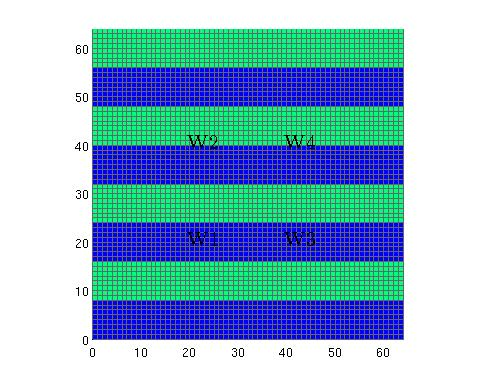
\includegraphics[width=4.3cm,height=4.3cm,keepaspectratio]{perm_he_1.jpg}
 \vspace{-20pt}
\caption{ Heterogeneous permeability, 4 wells.}\label{fig:hep}
\vspace{-15pt}
\end{wrapfigure}

\normalsize
As mentioned above, we studied flow through a porous medium with \emph{heterogeneous permeability} layers. A grid of
$nx = ny = 64$ elements is studied. We use 8 layers of the same size, 
4 layers with one value of permeability $\sigma_1$, followed by a layer with a different permeability value $\sigma_2$. Figure \ref{fig:hep} shows these layers. The permeability of one set of layers is set to $\sigma_1=1mD$, the permeability of the other set $\sigma_2$ is changed. 
Therefore, the contrast in permeability between the layers $(\frac{\sigma_2}{\sigma_1}=\frac{\sigma_2}{1mD})$,
depends on the value of $\sigma_2$.\\
We investigate the dependence on the contrast in permeability value between the layers for the ICCG and DICCG methods.
The permeability  $\sigma_2$ varies from $\sigma_2=10^{-1}mD$ to $\sigma_2=10^{-3}mD$. 
 The tolerance is set as $10^{-11}$ for the snapshots as well as for the original problem.\\
\renewcommand{\arraystretch}{1.3}
\begin{table}[!ht]\centering
\begin{minipage}{.65\textwidth}
\vspace{-20pt}
\centering
\begin{tabular}{ |c|c|c|c|} 
\hline
 $\kappa_2$ (mD) & $10^{-1}$& $10^{-2}$ & $10^{-3}$ \\
 \hline
  ICCG  & 75& 103&110\\ 
 
  DICCG  & 1 & 1& 1\\ 
 \hline
\end{tabular}
\caption{Table with the number of iterations for different contrasts in the permeability of the layers
for the ICCG and DICCG methods.}
\label{table:he}\end{minipage}
\vspace{-10pt}
\end{table}

 Table \ref{table:he} shows the number of iterations required to achieve convergence 
for ICCG and DICCG, for various permeability contrasts between the layers. \\
The plot of the residual and the solution 
to the problem are presented in Figures \ref{fig:convhe1} and \ref{fig:solhe1} for a value of permeability $\sigma_2=10^{-2}$.\\
We note that the number of 
iterations increases when the contrast between the permeability layers increases for ICCG. For DICCG, 
we observe that we only need one iteration despite the change in permeability contrast between the layers.
\begin{figure}[!h]
\centering
\begin{minipage}{.4\textwidth}
 \centering
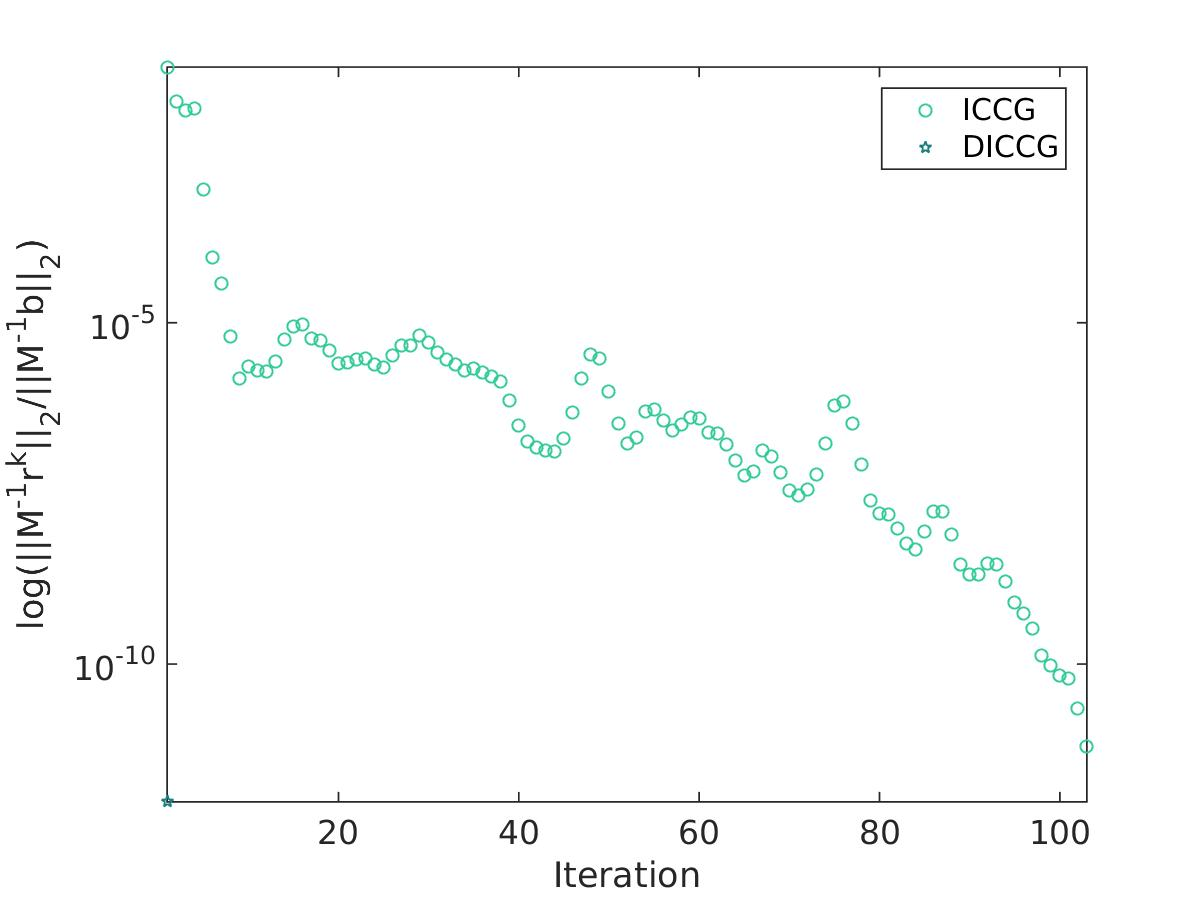
\includegraphics[width=5cm,height=5cm,keepaspectratio]
{conv_4w.jpg}
\caption{Convergence for the heterogeneous problem, 64 x 64 grid cells,  $\sigma_2=10^{-2}mD$.}
\label{fig:convhe1}
\end{minipage}%
\hspace{10pt}
\begin{minipage}{.4\textwidth} 
\centering 
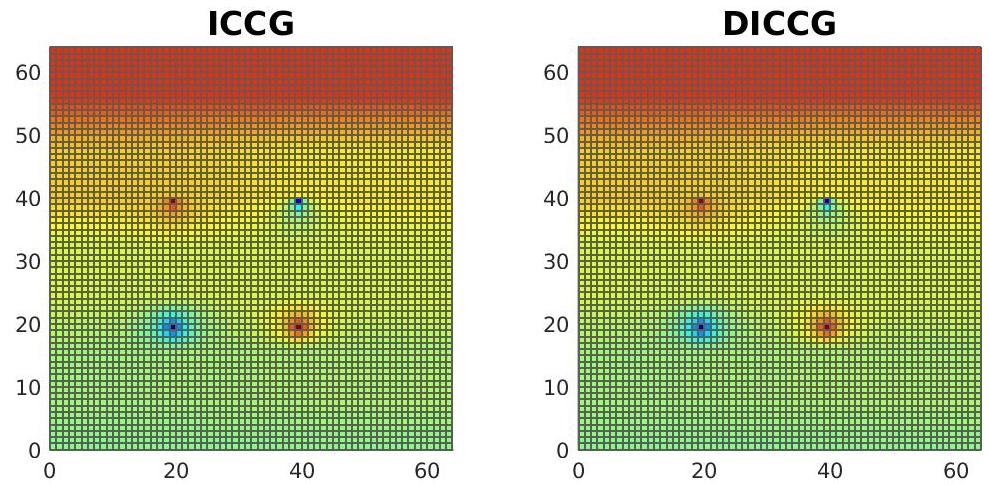
\includegraphics[width=6.5cm,height=6.5cm,keepaspectratio]
{sol_4w.jpg}
\caption{Solution of the heterogeneous problem, 64 x 64 grid cells, $\sigma_2=10^{-2}mD$.}
\label{fig:solhe1}
\end{minipage}
\end{figure}
%\begin{figure}[!h]
%\centering 
%\includegraphics[width=5cm,height=5cm,keepaspectratio]
%{perm_he_1.jpg}



\textbf{\emph{Case 2, Neumann boundary conditions only.}}\\
In this case, four wells are positioned in the corners and have a bhp of -1 bar. One well
is positioned in the center of the domain and has a bhp of +4 bars
(see Figure \ref{fig:hep1}). We set Neumann boundary conditions in all boundaries. For this case, we use a set of four linearly independent snapshots as deflation vectors. We also use a linearly dependent set of 15 snapshots and the basis of POD (linearly independent set) obtained from the 15 snapshots. We set the same boundary conditions as in the original problem for all the snapshots.
The four linearly independent snapshots ($z_1-z_4$) are obtained giving a value of zero to one well and non 
zero values to the other wells. The set of 15 snapshots are all the possible combinations of wells that satisfy that the flow in equals the flow out the reservoir (see section).
A summary of the configurations is presented below.
\newpage
\begin{itemize}
\item[] Configuration 2 :\\
\begin{minipage}{.6\textwidth}
\item[]  $System$ $configuration$ 
 \item[]  W1 =  W2 = W3 = W4 = -1 bar.
 \item[] W5 = +4 bars.
 \end{minipage}%
\begin{minipage}{.4\textwidth}
\item[] $Boundary$ $conditions:$\\
\item[] $\frac{\partial P(y=1)}{\partial n}=\frac{\partial P(y=ny)}{\partial n}=$
\item[] $\frac{\partial P(x=1)}{\partial n}=\frac{\partial P(x=nx)}{\partial n}=0$.
\end{minipage}
\begin{minipage}{.8\textwidth}
\item[] $Snapshots$ (4 linearly independent) 
 \item[] $\mathbf{z}_1$:  W2 = W3 = W4 =  -1 bars, 
 W1 = 0 bars, W5 = +3 bars.
\item[] $\mathbf{z}_2$: W1 = W3 = W4 = -1 bars,
 W2 = 0 bars, W5 = +3 bars.
\item[] $\mathbf{z}_3$: W1 = W2 = W4 = -1 bars,
 W3 = 0 bars, W5 =  +3 bars.
\item[] $\mathbf{z}_4$:  W1 = W2 = W3 = -1 bars,
 W4 = 0 bars, W5 =  +3 bars.
\item[] Dependent snapshots
\item[] $\mathbf{z}_5$: W1 = W2 = W3 = W4 =  -1 bars, 
 W5 =  +4 bars.
\item[] $\mathbf{z}_6$: W1 = W2 = 0 bars,
 W3 = W4 = -1 bars, W5 =  +2 bars.
\item[] $\mathbf{z}_7$: W2 = W3 = 0 bars, 
 W1 = W4 = -1 bars, W5 = +2 bars.
\item[] $\mathbf{z}_8$: W3 = W4 = 0 bars, 
 W1 = W2 = -1 bars, W5 =  +2 bars.
 \item[] $\mathbf{z}_9$: W1 = W3 = 0 bars, 
 W2 = W4 =  -1 bars, W5 = +2 bars.
\item[] $\mathbf{z}_{10}$: W2 = W4 = 0 bars, 
 W1 = W3 = -1 bars, W5 =  +2 bars.
\item[] $\mathbf{z}_{11}$: W1 = W4 = 0 bars, 
 W2 = W3 = -1 bars, W5 = +2 bars.
 \item[] $\mathbf{z}_{12}$: W1 = -1 bars, W2 = W3 = W4 =  0 bars, 
 W5 =  +1 bars.
\item[] $\mathbf{z}_{13}$: W2 = -1 bars, W1 = W3 = W4 = 0 bars,
 W5 = +1 bars.
\item[] $\mathbf{z}_{14}$: W3 = -1 bars, W1 = W3 = W4 = 0 bars,
 W5 = +1 bars.
\item[] $\mathbf{z}_{15}$: W4 = -1 bars, W1 = W2 = W3 = 0 bars,
 W5 =  +1 bars.
\end{minipage}%
\end{itemize}
\normalsize

\emph{Heterogeneous permeability layers}\\

\begin{wrapfigure}{R}{4.3cm}
\centering 
\vspace{-10pt}
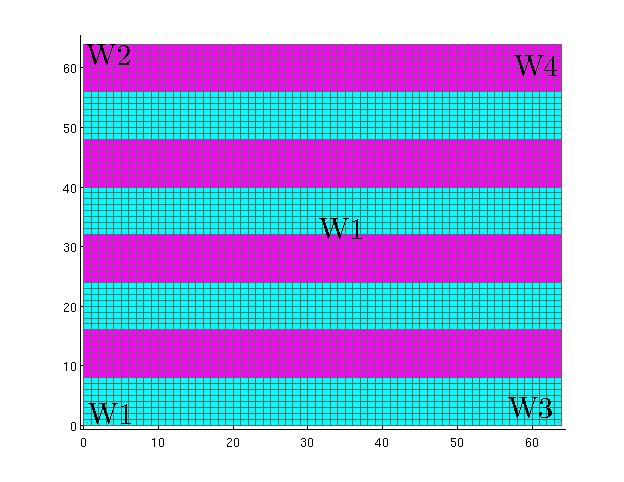
\includegraphics[width=4.3cm,height=4.3cm,keepaspectratio]{perm_he_2.jpg}
 \vspace{-25pt}
\caption{ Heterogeneous permeability, 5 wells.}\label{fig:hep_2}
\vspace{-15pt}
\end{wrapfigure} 
As in the previous case, single-phase flow through a porous medium with heterogeneous permeability layers is studied.
A grid of $nx = ny = 64$ elements is investigated. The deflation vectors used in this case are the 4 snapshots ($\mathbf{z}_1$-$\mathbf{z}_4$), a set of 15 linearly dependent vectors and basis vectors obtained for the POD method from the latter set.\\
The snapshots and the solutions are obtained with a tolerance of $10^{-11}$. \\
\begin{figure}[!ht]
%\begin{wrapfigure}{R}{5cm}
\vspace{-20pt}
 \centering
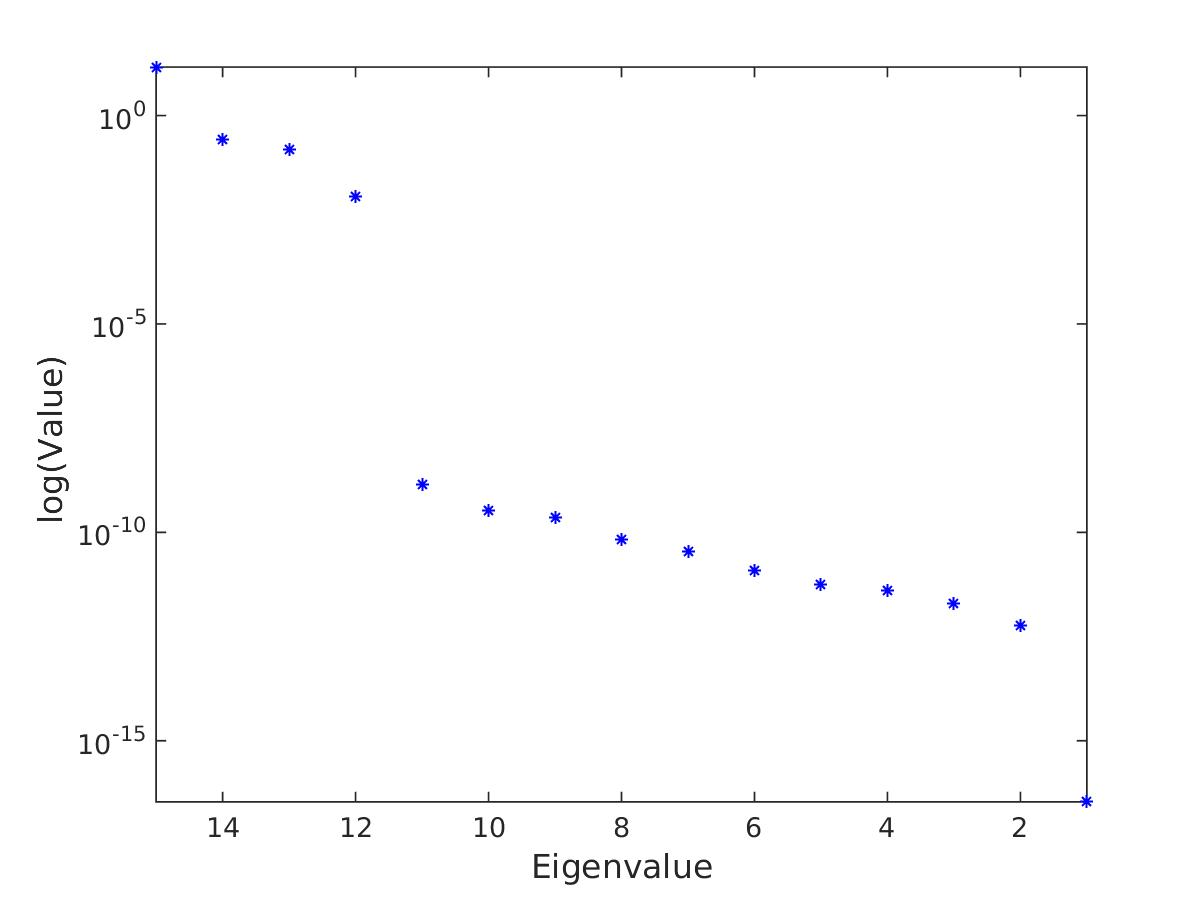
\includegraphics[width=7cm,height=7cm,keepaspectratio]
{eig_pod_5w.jpg}
\vspace{-10pt}
\caption{Eigenvalues of the snapshot correlation matrix $\mathbf{R}=\mathbf{X}\mathbf{X}^T$, 15 snapshots used.}
\vspace{-20pt}
\label{fig:eig}
%\end{wrapfigure}
\end{figure} 
Table \ref{table:he2} shows the number of iterations required to reach convergence for ICCG method and the deflation method with four linearly independent snapshots as deflation vectors DICCG$_{4}$, 15 linearly dependent snapshots DICCG$_{15}$ and the basis vectors of POD, DICC$G_{POD}$\footnote{The * means that the solution is not reached.}. 
For the selection of the deflation vectors of DICCG$_{POD}$ we plot the eigenvalues of the snapshot correlation matrix $\mathbf{R}=\mathbf{X}^T \mathbf{X}$ (see section ) in Figure \ref{fig:eig}. We observe that there are 4 eigenvalues larger than the rest of the eigenvalues which are the responsible of hamper the convergence of the method, therefore we use the eigenvectors corresponding to these eigenvalues as deflation vectors.\\
The plot of the residual and the solution of the problem are presented in
Figure \ref{fig:convhe2} and \ref{fig:solhe2} for the ICCG and DICCG methods for the case of $\sigma_2=10^{-1}$.\\
\renewcommand{\arraystretch}{1.3}
\begin{table}[!ht]\centering
\begin{minipage}{.8\textwidth}
\vspace{-10pt}
\centering
\begin{tabular}{ |c|c|c|c|} 
\hline
 $\sigma_2$ (mD) & $10^{-1}$& $10^{-2}$ & $10^{-3}$ \\
 \hline
  ICCG  & 90& 115&131\\ 
 
  DICCG$_4$  & 1 & 1& 1\\ 
  DICCG$_{15}$  & 200* & 200*& 200*\\
  DICCG$_{POD}$  & 1 & 1& 1\\
 \hline
\end{tabular}
\caption{Table with the number of iterations for different contrast in the permeability of the layers
for the ICCG, DICCG$_4$, DICCG$_{15}$, and DICCG$_{POD}$ methods, tolerance of solvers and snapshots $10^{-11}$.}
\label{table:he2}\end{minipage}
\vspace{-10pt}
\end{table}

For the ICCG method, we observe that the number of iterations 
increases as the contrast in the permeability increases. For the DICCG method with 4 linearly independent deflation vectors and 4 basis vectors of POD, convergence is reached 
within one iteration. However, for the case of 15 linearly dependent vectors, the solution is not reached within the 200 iterations allowed for this problem.\\


\begin{figure}[!h]
\centering
\begin{minipage}{.4\textwidth}
 \centering
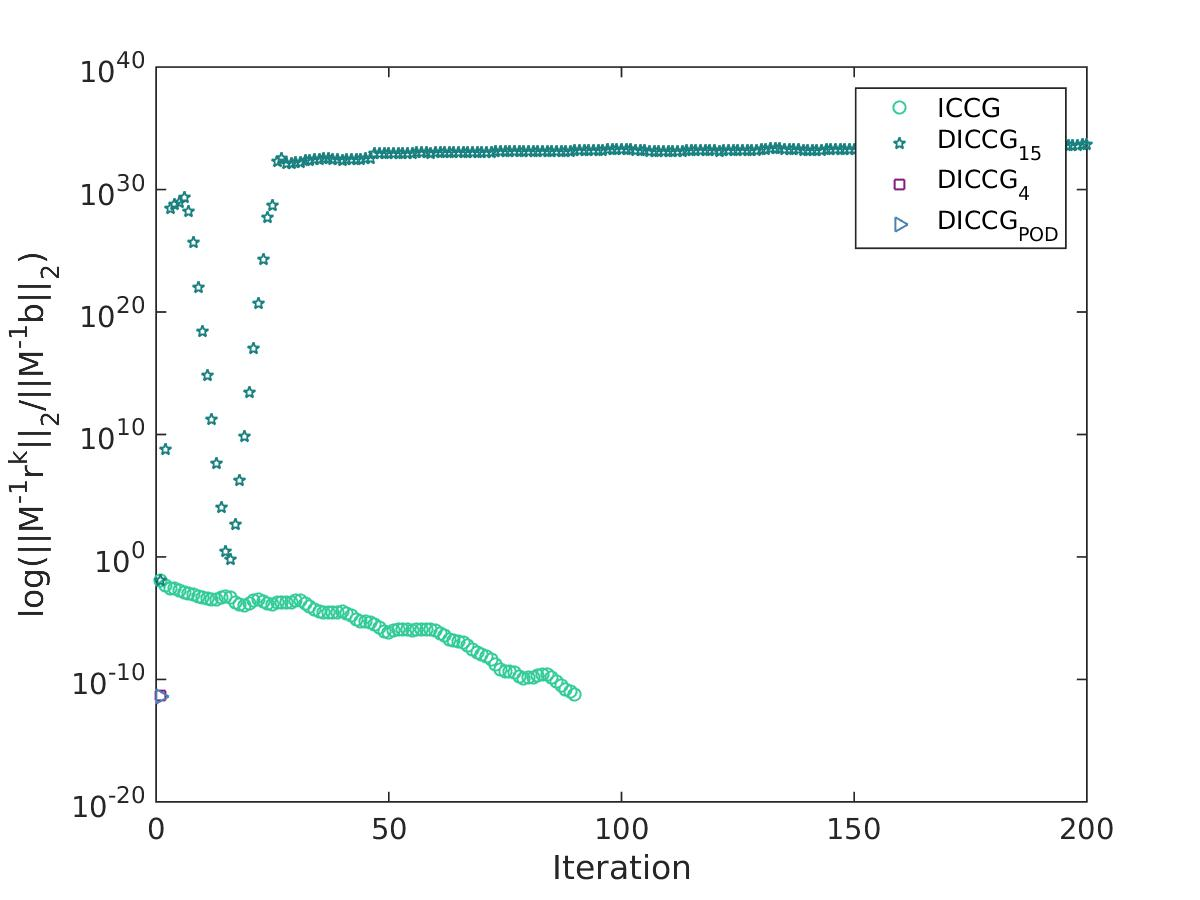
\includegraphics[width=6.5cm,height=6.5cm,keepaspectratio]
{conv_5w.jpg}
\caption{Convergence for the heterogeneous problem, 64 x 64 grid cells, $\sigma_2=10^{-1}$.}
\label{fig:convhe2}
\end{minipage}%
\hspace{10 pt}
\begin{minipage}{.4\textwidth}
 \centering
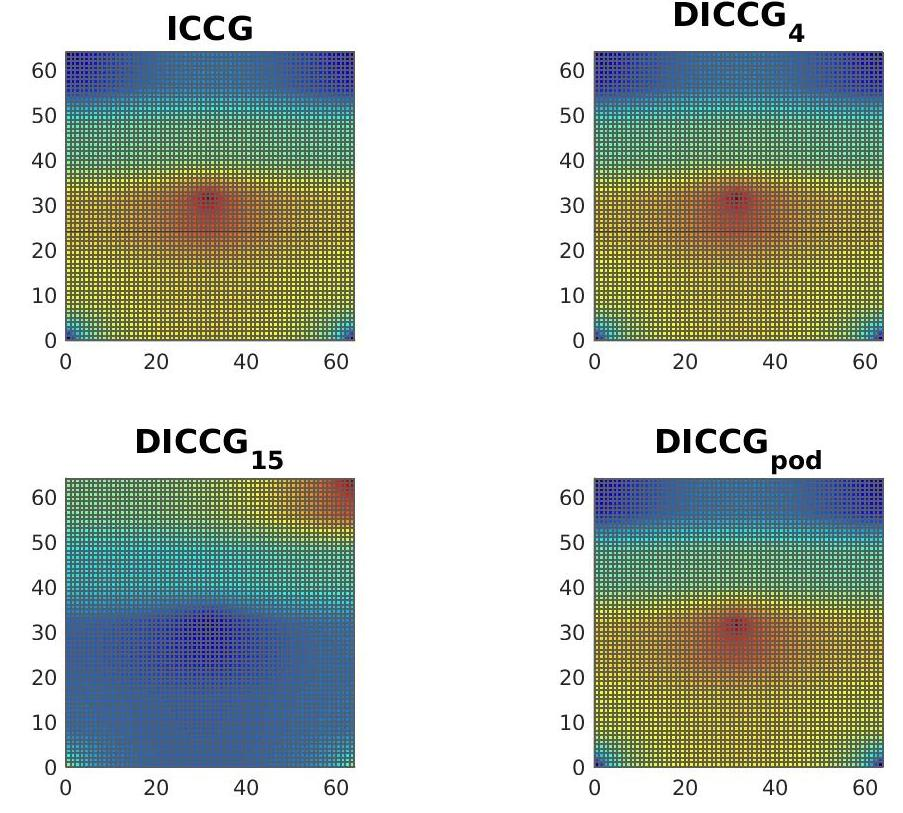
\includegraphics[width=5cm,height=5cm,keepaspectratio]
{sol_5w.jpg}
\caption{Solution of the heterogeneous problem, 64 x 64 grid cells, $\sigma_2=10^{-1}$.}
\label{fig:solhe2}
\end{minipage}
\end{figure}

\newpage
\emph{SPE 10 model}\\
This model has large variations in the permeability coefficients, $\mathcal{O} (10^7)$.
It has 5 sources or wells, four producers in the corners (negative) and one injector in the center (positive).
The model contains 60 x 220 x 85 cells, we study the dependence of the ICCG and the DICCG method on the size of the problem. One layer is studied with various grid sizes 16 x 56, 30 x 110, 46 x 166 and 60 x 220, and the complete model containing 85 layers.
Permeability is upscaled
averaging the permeability in each grid using the harmonic-arithmetic average algorithm from MRST.
The permeability of the coarser grid (16 x 56 cells) is shown in Figure \ref{fig:permc} and the complete model in Figure \ref{fig:permcc}.
The permeability contrast for the diverse grid size problems is shown in Table \ref{table:permgs}. From this table, we observe that the contrast in the permeability for different grid sizes varies slightly, but that the order
of magnitude remains the same for all the cases.\\
\\The snapshots are obtained solving the system with different well
configurations (\emph{Configuration 2}). As before, we simulate single-phase incompressible flow.\\
The system and snapshots are solved with an accuracy of $10^{-7}$.
In the first experiment with the deflation method, the four linearly independent snapshots are used as deflation vectors (DICCG). Then, 
15 linearly dependent vectors and finally 4 vectors of the POD basis are used as deflation vectors (DICCG$_{POD}$). \\ 
\begin{figure}[!h]
\centering
\begin{minipage}{.4\textwidth}
 \centering
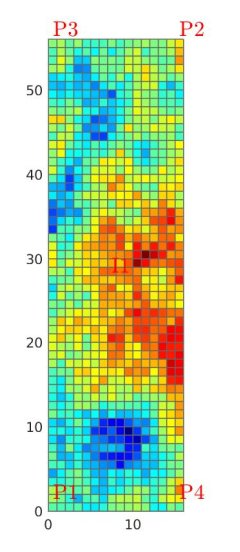
\includegraphics[width=4.5cm,height=4.5cm,keepaspectratio]
{perm_layer_2.jpg}
\caption{SPE 10 benchmark, 2nd layer 16 x 56 grid cells, permeability field.}
\label{fig:permc}
\end{minipage}%
\hspace{4mm}
\begin{minipage}{.4\textwidth}
 \centering
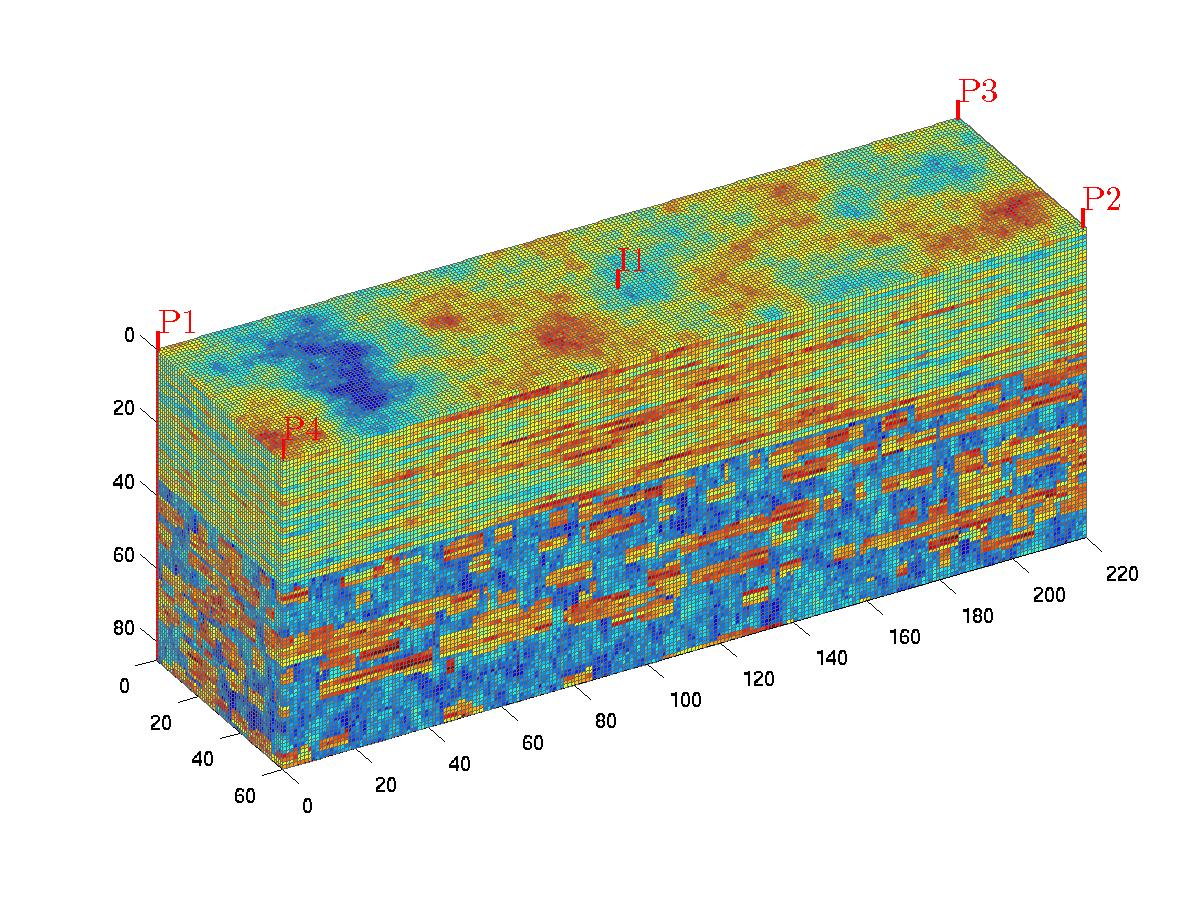
\includegraphics[width=5.5cm,height=5.5cm,keepaspectratio]
{perm_layer_.jpg}
\caption{SPE 10 benchmark, permeability field.}
\label{fig:permcc}
\end{minipage}
\end{figure}


\begin{table}[!ht]
\centering
\begin{tabular}{ |c|c|c|c|c|c|  } 
 \hline
  Grid size & 16x56x1& 30x110x1& 46x166x1& 60x220x1&60x220x85\\
  \hline
  Contrast ($\times10^{7}$) & 1.04 & 2.52&  2.6&  2.8 &3\\ 
\hline
\end{tabular}
\caption{Table with the contrast of permeabilities for
different grid sizes.}
\label{table:permgs}
\end{table}

The number of iterations required to achieve convergence with the ICCG and DICCG methods for various
grid sizes is presented in Table \ref{table:itgrid}. \\
As in the previous experiment, the number of iterations is similar for the DICCG and DICCG$_{POD}$ methods,
therefore we will analyze only the solutions obtained with DICCG, as the same analysis holds for DICCG$_{POD}$.
\\The convergence and the solution to the ICCG and DICCG methods are presented in Figure \ref{fig:convspe} and Figure \ref{fig:solspe} for the complete problem. 
For ICCG, the required iterations to reach convergence increases as the size of the grid increases. Meanwhile, for the deflated methods only one iteration is required and it does not change with the size of the grid.
We can also note that for the deflated method with 15 linearly dependent snapshots as deflation vectors (DICCG$_{15}$), after the first iteration, the relative residual is close to two orders of magnitude larger than for the other deflation methods (DICCG$_{4}$, DICCG$_{POD}$).   

\begin{table}[!ht]
\centering
\begin{tabular}{|c |c|c|c|c|c| c| } 
 \hline
Method  & 16x56x1& 30x110x1& 46x166x1& 60x220x1&60x220x85\\
   \hline
  ICCG & 34 & 74&  128 &  162&357 \\ 
   DICCG$_{15}$ & 1 & 1&  1 &  1& 3\\ 
   DICCG$_{4}$ & 1 & 1&  1 &  1& 1\\  
   DICCG$_{POD}$ & 1 & 1&  1 &  1 &1\\ 
\hline
\end{tabular}
\caption{Table with the number of iterations for ICCG and DICCG methods, various tolerance for the snapshots,
various grid sizes.}
\label{table:itgrid}
\end{table}
\begin{figure}[!h]
\centering
\begin{minipage}{.5\textwidth}
 \centering
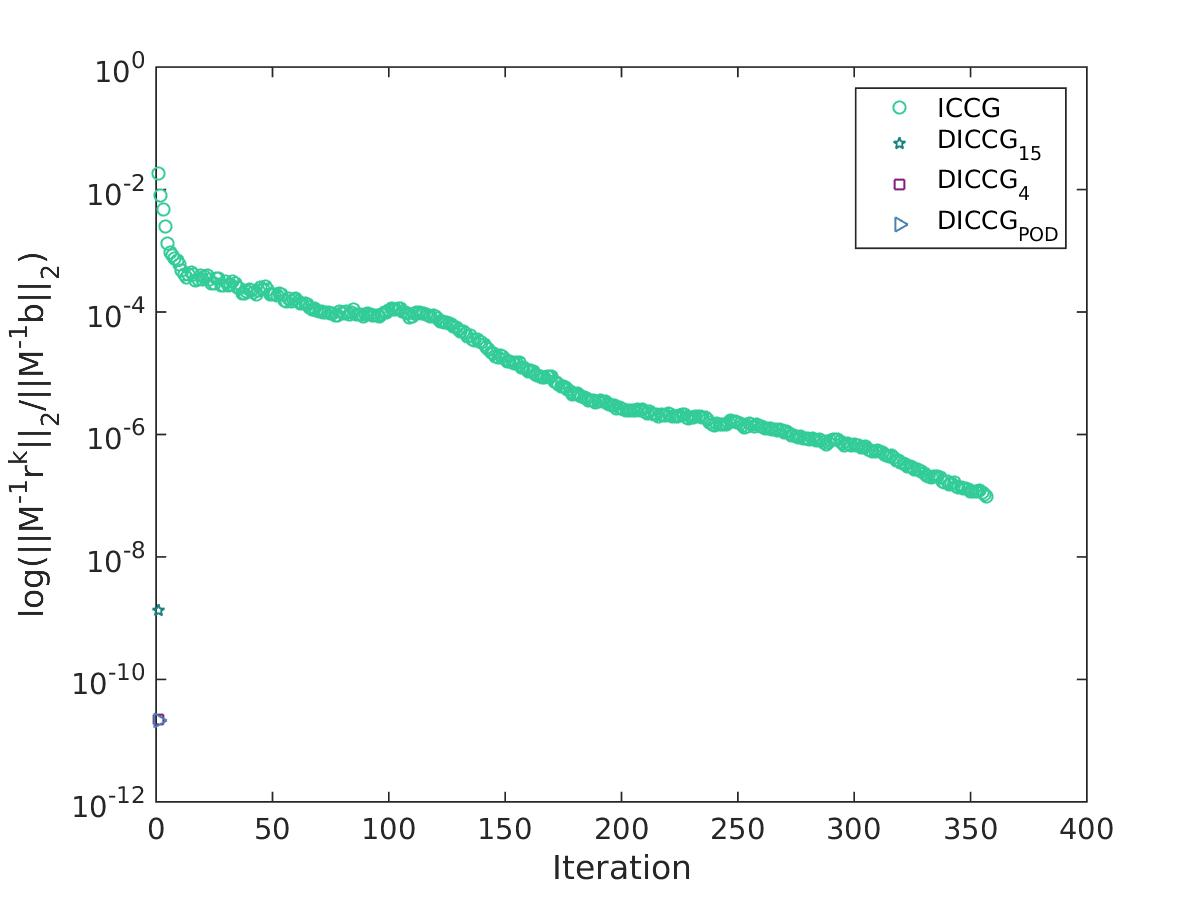
\includegraphics[width=7cm,height=7cm,keepaspectratio]
{conv_spe10c.jpg}
\caption{Convergence for the SPE 10 problem, 60 x 220 x 85 grid cells, accuracy of the snapshots $10 ^{-7}$.}
\label{fig:convspe}
\end{minipage}%
\hspace{4mm}
\begin{minipage}{.45\textwidth}
 \centering
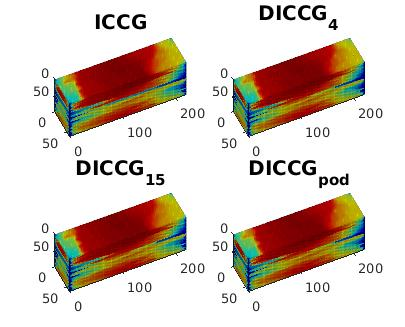
\includegraphics[width=6cm,height=6cm,keepaspectratio]
{sol_spe10c.jpg}
\caption{Solution of the SPE 10 benchmark, 16 x 56 grid cells, 2nd layer, accuracy of the snapshots $10 ^{-7}$.}
\label{fig:solspe}
\end{minipage}
\end{figure}
\newpage

\newpage
\subsection*{Compressible Problem}

\begin{wrapfigure}{R}{5cm}
\centering 
\vspace{-10pt}
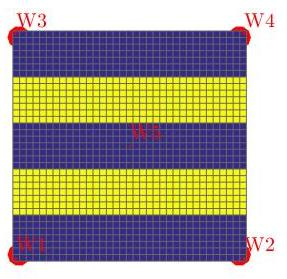
\includegraphics[width=4.5cm,height=4.5cm,keepaspectratio]{perm_comp.jpg}
 \vspace{-5pt}
\caption{ Heterogeneous permeability, 5 wells, compressible problem.}\label{fig:pc}
\vspace{-15pt}
\end{wrapfigure} 
For this problem, we solve \eqref{eq:peace} where $\mathbf{V}$ depends on the pressure according to Equation (\eqref{}). 
A grid of $35\times 35$ cells is used with Newmann boundary conditions only. The domain consist of layers with two different permeability values (see Figure \ref{fig:pc}). The first layer has a permeability of $\sigma_1 = 30mD$, and the permeability of the second layer is $\sigma_2 = 3mD$. Therefore the permeability contrast between the layers is $10^{-1}$.The initial pressure of the reservoir is set as 200 bars. Four wells are positioned in the corners of the domain with a bhp of 100 bars, and a well is placed in the center of the domain with a bhp of 600 bars.
 For the first set of problems, we use the solution of the first 10 time steps with the same configuration as the problem as deflation vectors. We solve the rest of the time steps with DICCG$_{10}$ method with the 10 snapshots as deflation vectors and with 5 basis POD vectors as deflation vectors, DICCG$_{POD}$.
 For the second set of experiments, we use the same configuration as in the original problem but we vary the configuration of the wells. One corner well has the same pressure as the reservoir (200 bar), the other corner wells have a pressure of 100 bars and the central well has a pressure of 500 bars. 

\begin{itemize}
\begin{minipage}{.6\textwidth}
\item[]  $System$ $configuration$
\item[] Initial pressure 200 bar.
 \item[]  W1 =  W2 = W3 = W4 = 100 bar.
 \item[] W5 = 600 bars.\\
 \end{minipage}%
\begin{minipage}{.4\textwidth}
\item[] $Boundary$ $conditions:$\\
\item[] $\frac{\partial P(y=1)}{\partial n}=\frac{\partial P(y=ny)}{\partial n}=$
\item[] $\frac{\partial P(x=1)}{\partial n}=\frac{\partial P(x=nx)}{\partial n}=0$.
\end{minipage}
\begin{minipage}{.8\textwidth}
\item[] $Snapshots (second set of experiments)$ 
 \item[] $\mathbf{z}_1$:  W2 = W3 = W4 =  100 bars, 
 W1 = 200 bars, W5 = 500 bars.
\item[] $\mathbf{z}_2$: W1 = W3 = W4 = 100 bars,
 W2 = 200 bars, W5 = 500 bars.
\item[] $\mathbf{z}_3$: W1 = W2 = W4 = 100 bars,
 W3 = 200 bars, W5 =  500 bars.
\item[] $\mathbf{z}_4$:  W1 = W2 = W3 = 100 bars,
 W4 = 200 bars, W5 =  500 bars.\\
\end{minipage}%
\end{itemize}
The simulation was performed during 152 days with 52 time steps and a time step of 3 days. The tolerance of the NR method and the linear solvers was of $10^{-5}$.\\
\emph{\textbf{Case 1}}\\
In Figure \ref{fig:compsol}, the solution obtained with ICCG method is presented, the solution is the same for all methods. The upper left figure represents the pressure field at the final time step. The upper right figure represents the pressure across the diagonal joining the (0,0) and (35,35) grid cells. We observe the initial pressure (200 bars) in this diagonal and the evolution of the pressure field through the time. In the lower figure we observe the surface volume rate for the five wells during the simulation.\\
\begin{figure}[!h]
\centering
\begin{minipage}{.7\textwidth}
 \centering
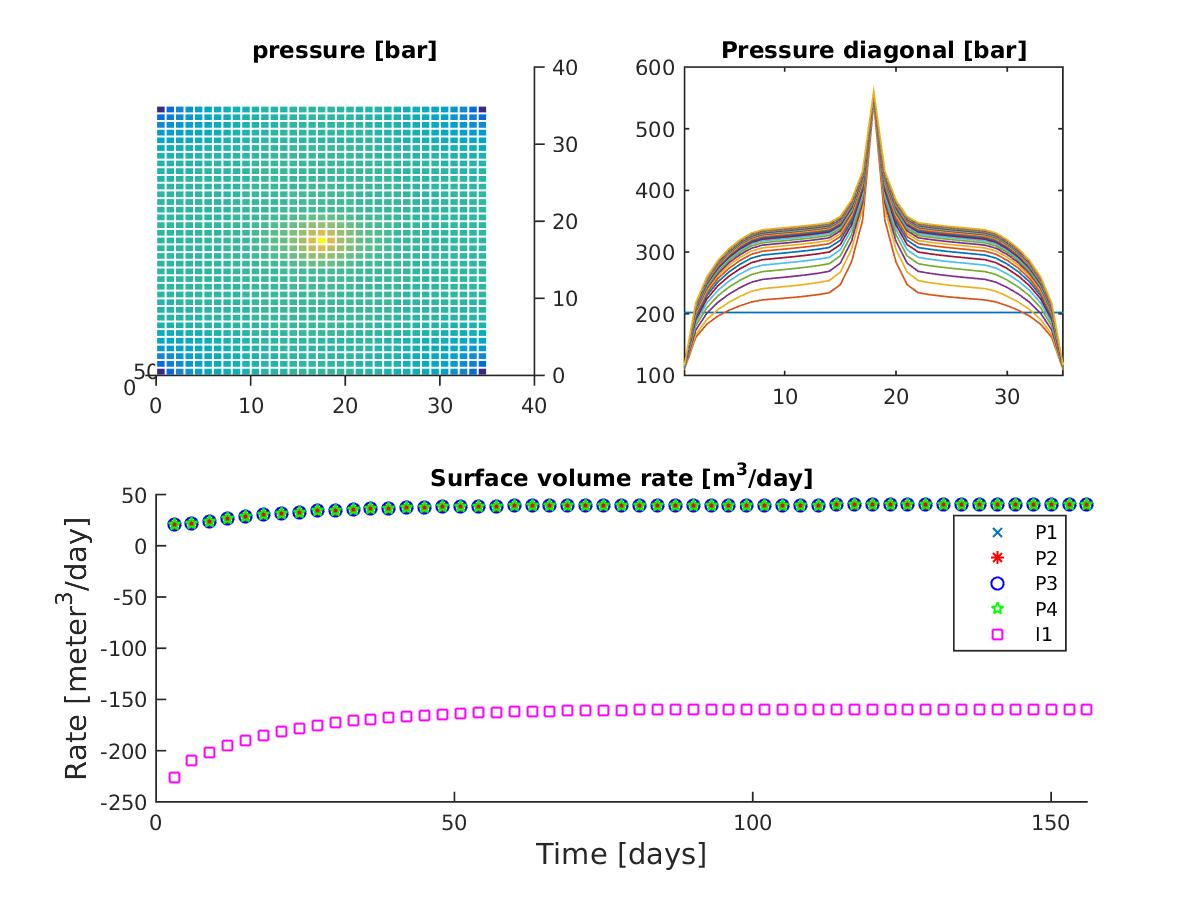
\includegraphics[width=10cm,height=10cm,keepaspectratio]
{solutionIC.jpg}
\caption{Solution of the compressible problem solved with the ICCG method.}
\label{fig:compsol}
\end{minipage}
\end{figure}

The number of iterations necessary to reach convergence with the linear solvers is presented for the first four NR iterations in Figure \ref{fig:NR_IC} for the ICCG method, Figure \ref{fig:NR_D10} for the deflated method DICCG$_{10}$ using 10 snapshots as deflation vectors and Figure \ref{fig:NR_POD5} DICCG$_{POD}$ using 5 basis vectors of POD as deflation vectors. 
\begin{figure}[!h]
\centering
\begin{minipage}{.4\textwidth}
 \centering
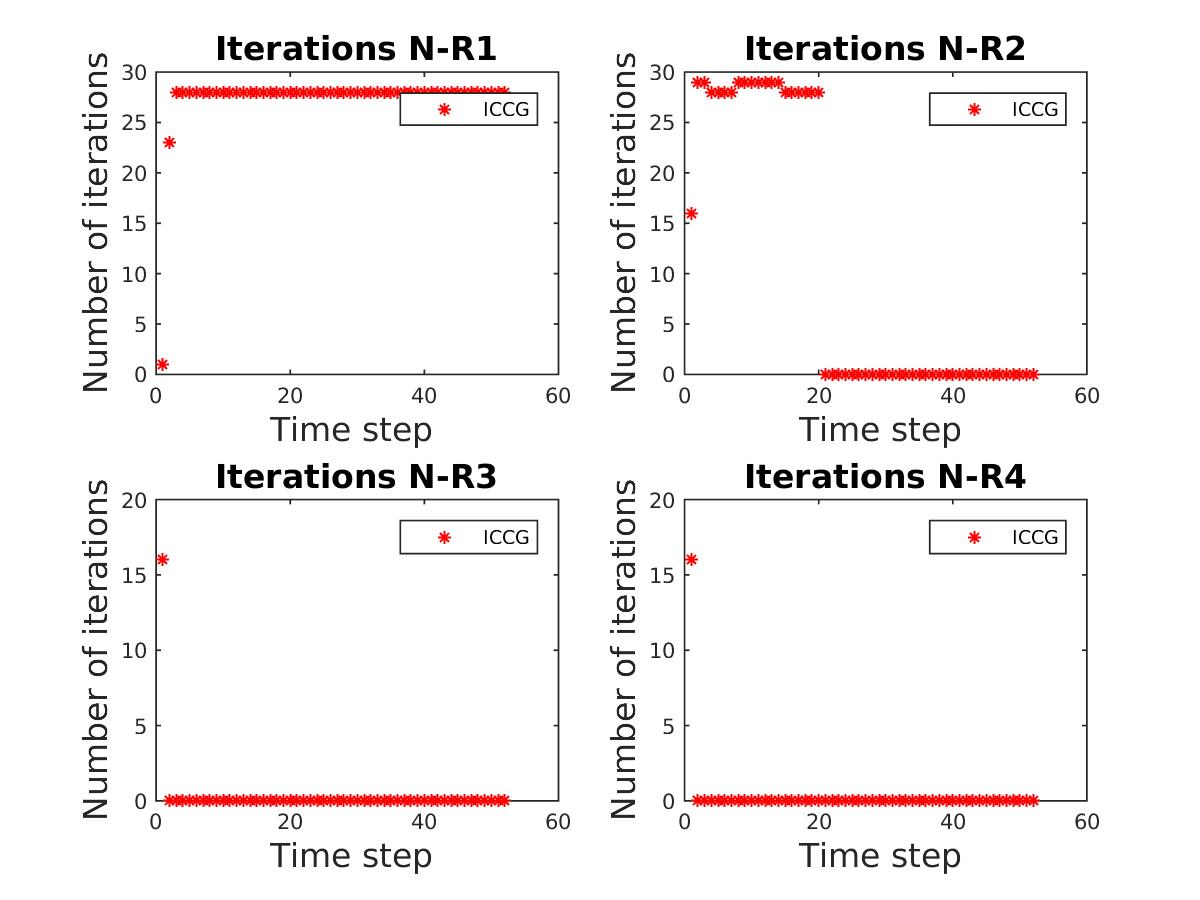
\includegraphics[width=6.5cm,height=6.5cm,keepaspectratio]
{iterations_4NR_IC.jpg}
\caption{Number of iterations of the ICCG method for the first four NR iterations.}
\label{fig:NR_IC}
\end{minipage}
\end{figure}

\begin{figure}[!h]
\centering
\begin{minipage}{.4\textwidth}
 \centering
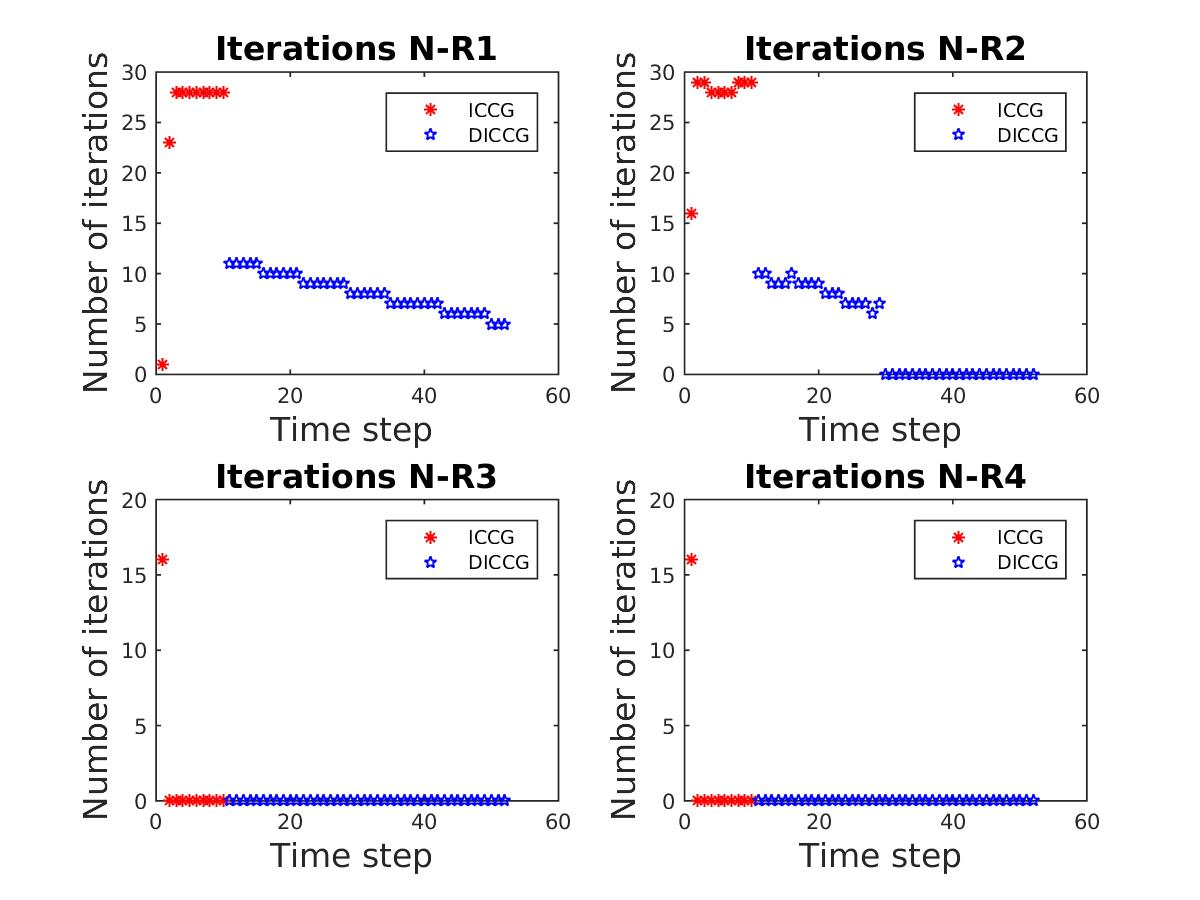
\includegraphics[width=6.5cm,height=6.5cm,keepaspectratio]
{iterations_4NR_D10.jpg}
\caption{Number of iterations of the DICCG$_{10}$ method for the first four NR iterations.}
\label{fig:NR_D10}
\end{minipage}%
\hspace{15mm}
\begin{minipage}{.4\textwidth}
 \centering
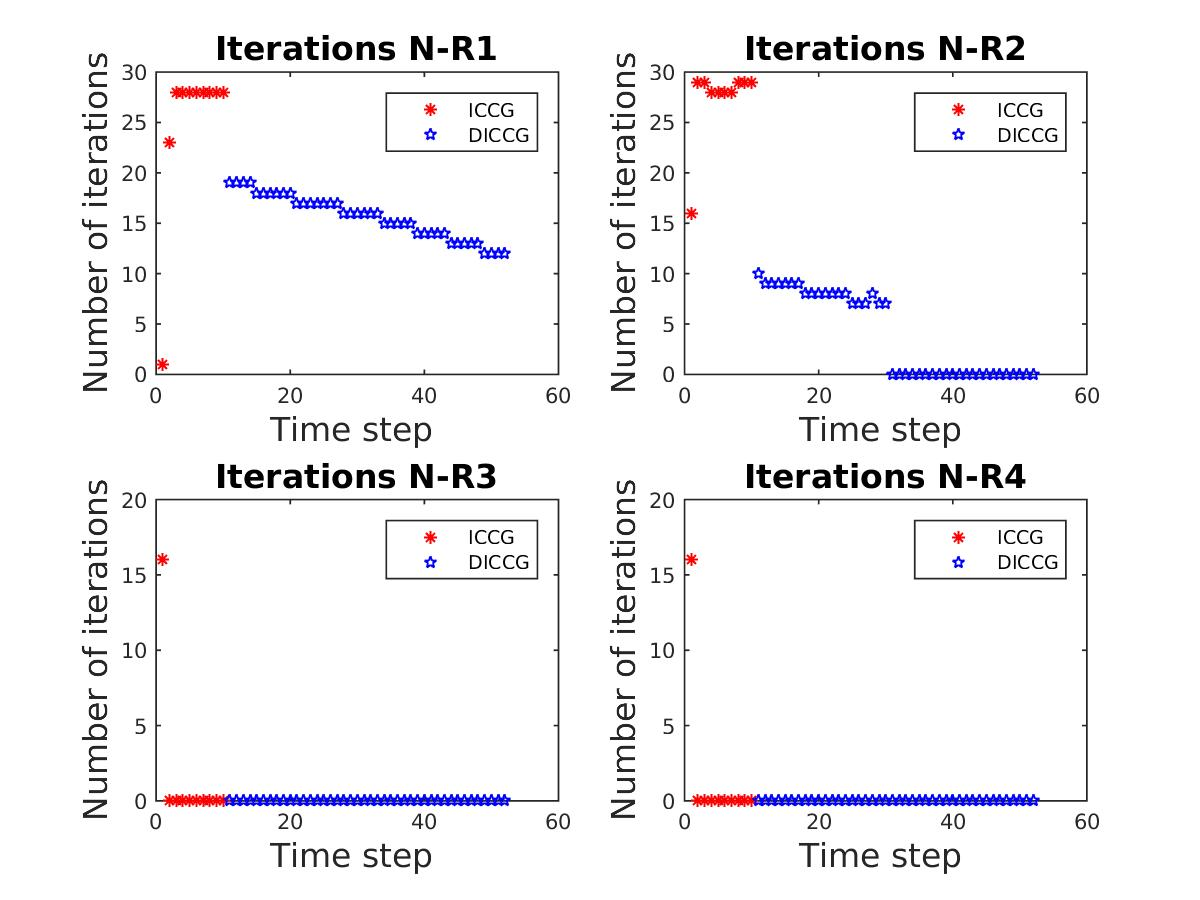
\includegraphics[width=6.5cm,height=6.5cm,keepaspectratio]
{iterations_4NR_POD5.jpg}
\caption{Number of iterations of the DICCG$_{POD}$ method for the first four NR iterations.}
\label{fig:NR_POD5}
\end{minipage}
\end{figure}
We observe that the number of iterations for the first and second NR iterations is lower for the deflated methods compared with the ICCG method. However, we observe that the time step when convergence is achieved for the NR cycle is larger for these methods with respect to the ICCG method. We also observe that for the first NR iteration, the decrease is larger for the deflated method with 10 snapshots as deflation vectors.\\
\emph{\textbf{Case 2}}\\
In the second case, we compute the first 4 time steps varying the bhp of the wells, as described above. Figure \ref{fig:compsolvw} presents the solution obtained with ICCG method is presented. The upper left figure represents the pressure field at the final time step. The upper right figure represents the pressure across the diagonal joining the (0,0) and (35,35) grid cells. We can observe the initial pressure (200 bars) in this diagonal and the evolution of the pressure field through the time. In the lower figure we observe the surface volume rate for the five wells during the simulation.

\begin{figure}[!h]
\centering
\begin{minipage}{.7\textwidth}
 \centering
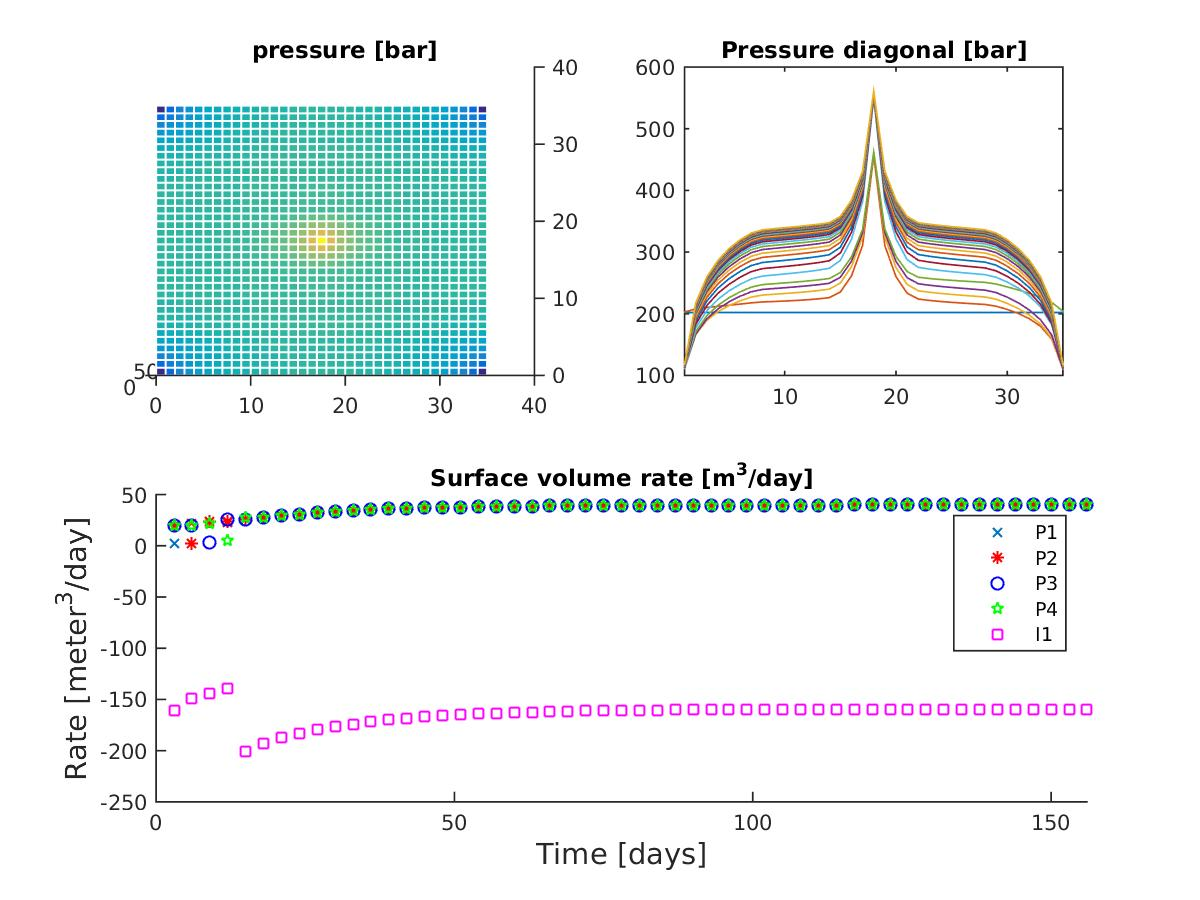
\includegraphics[width=10cm,height=10cm,keepaspectratio]
{solutionvw_IC.jpg}
\caption{Solution of the compressible problem solved with the ICCG method, varying the bhp of the first 4 time steps.}
\label{fig:compsolvw}
\end{minipage}
\end{figure}
The number of iterations necessary to achieve convergence with the linear solvers for this second problem is presented for the first four NR iterations in Figure \ref{fig:vwNR_IC} for the ICCG method, Figure \ref{fig:vwNR_D10} for the deflated method DICCG$_{10}$ using 10 snapshots as deflation vectors and Figure \ref{fig:vwNR_POD5} DICCG$_{POD}$ using 5 basis vectors of POD as deflation vectors. 
\begin{figure}[!h]
\centering
\begin{minipage}{.4\textwidth}
 \centering
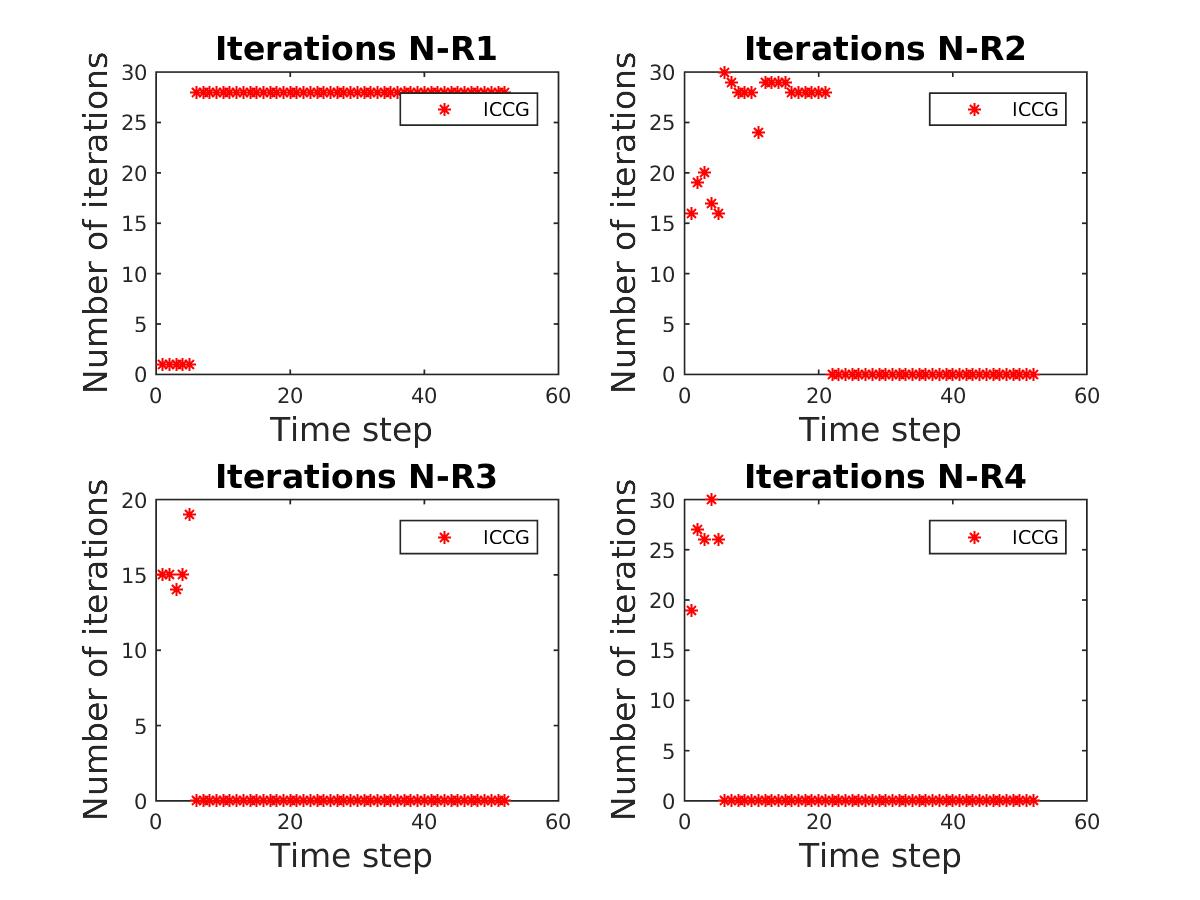
\includegraphics[width=6.5cm,height=6.5cm,keepaspectratio]
{iterations_4NRvw_IC.jpg}
\caption{Number of iterations of the ICCG method for the first four NR iterations.}
\label{fig:vwNR_IC}
\end{minipage}
\end{figure}

\begin{figure}[!h]
\centering
\begin{minipage}{.4\textwidth}
 \centering
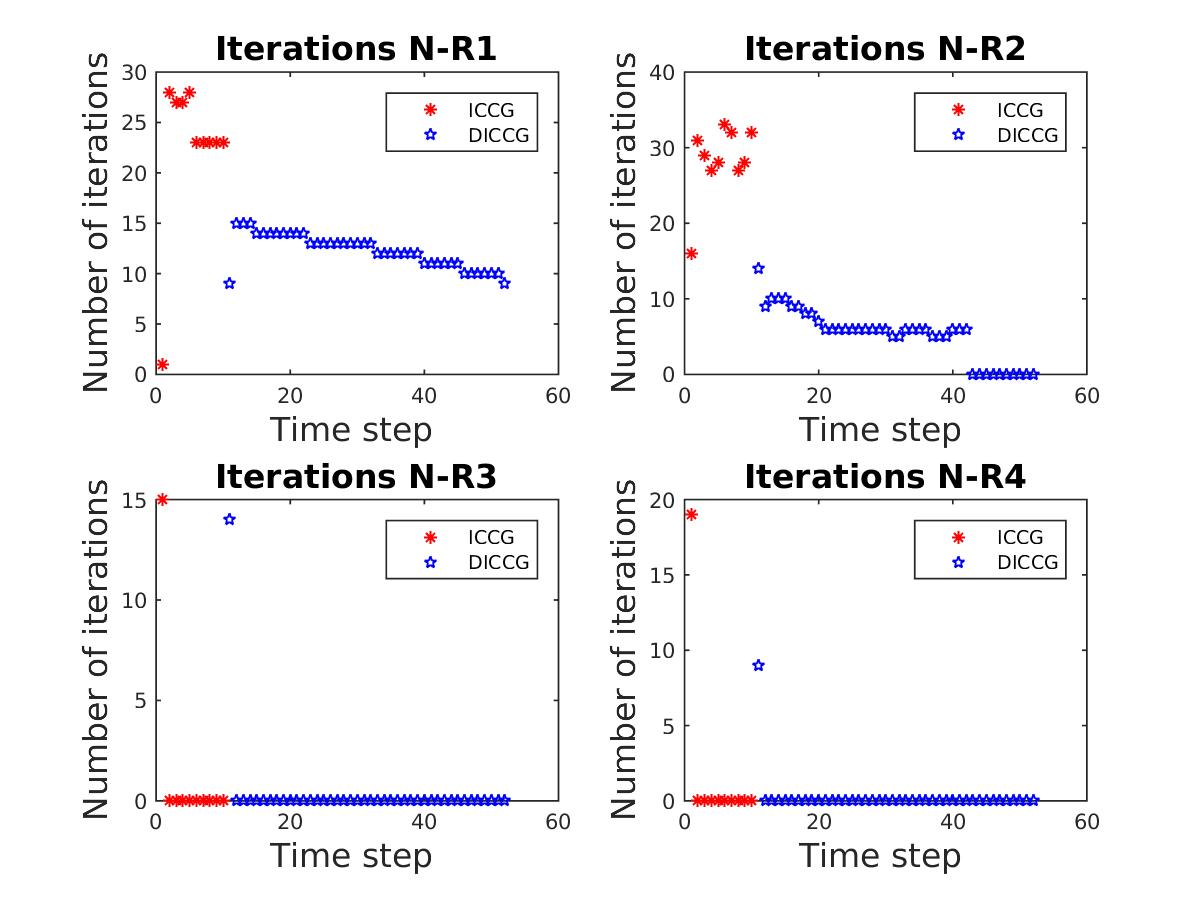
\includegraphics[width=6.5cm,height=6.5cm,keepaspectratio]
{iterations_4NRvw_D10.jpg}
\caption{Number of iterations of the DICCG$_{10}$ method for the first four NR iterations.}
\label{fig:vwNR_D10}
\end{minipage}%
\hspace{15mm}
\begin{minipage}{.4\textwidth}
 \centering
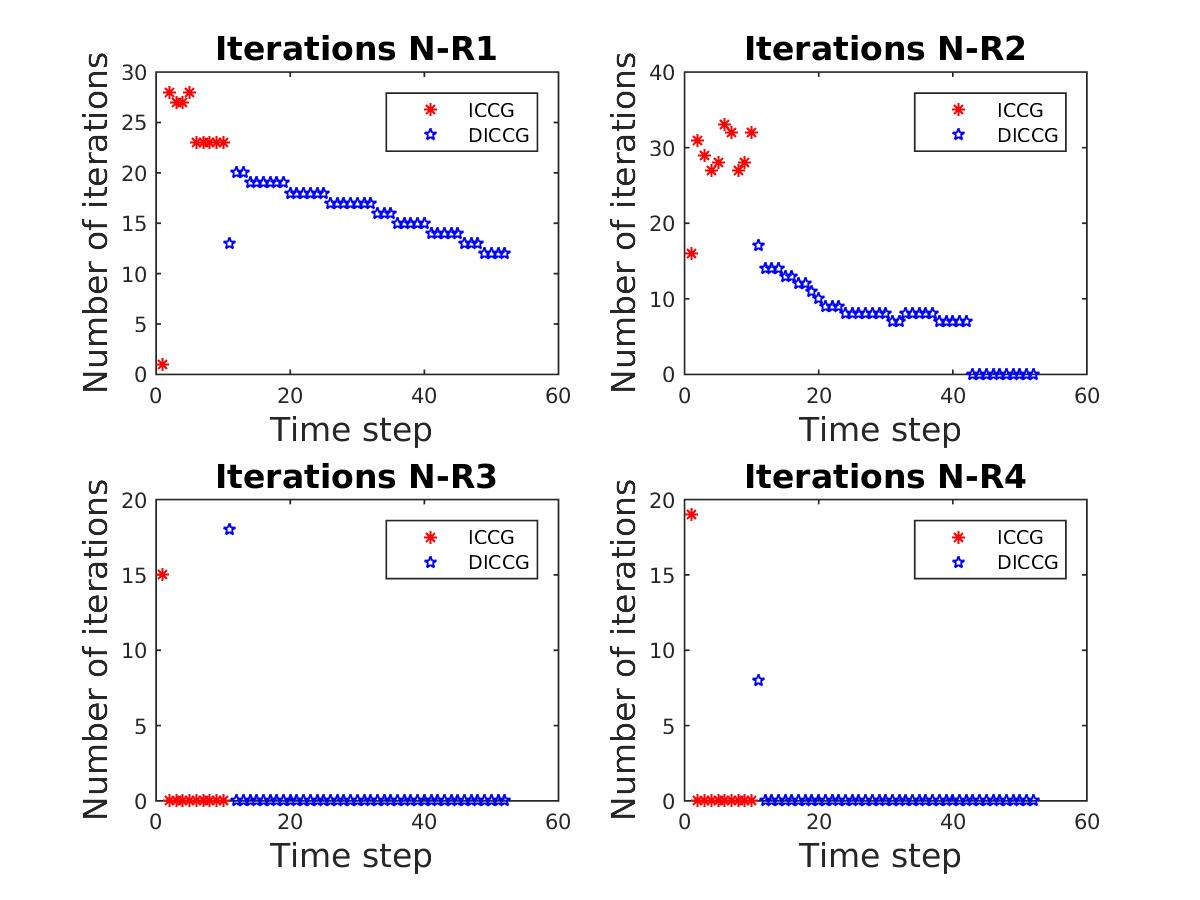
\includegraphics[width=6.5cm,height=6.5cm,keepaspectratio]
{iterations_4NRvw_POD5.jpg}
\caption{Number of iterations of the DICCG$_{POD}$ method for the first four NR iterations.}
\label{fig:vwNR_POD5}
\end{minipage}
\end{figure}
As in the previous case, we observe that the number of iterations for the first and second NR iterations is lower for the deflated methods compared with the ICCG method. However, we observe that the time step when convergence is achieved for the NR cycle is larger for these methods with respect to the ICCG method. We also observe that for the first NR iteration, the reduction is larger for the deflated method with 10 snapshots as deflation vectors.


\newpage
\newpage
\bibliographystyle{unsrt}
\bibliography{research}

\end{document}